\documentclass[10pt]{article}
\usepackage[obeyspaces]{url}
\usepackage{fancyvrb}
\usepackage{graphicx}
\usepackage{mathptmx}
\usepackage{courier}
\usepackage[scaled=.90]{helvet}
\usepackage{comment}
%\usepackage[body={6.5in, 9.0in},left=1.0in, nohead]{geometry}
%\usepackage{setspace}
%\onehalfspacing
% change figure placement behavior
\renewcommand{\topfraction}{0.85}
\renewcommand{\textfraction}{0.1}
\usepackage{paralist}
% paragraph adjustment
%\setlength{\parindent}{0pt}
%\setlength{\parskip}{0.25cm}

%%%% redefine url to make courier OK
\renewcommand{\UrlFont}{\small\tt}
%%%% running head
\newcommand{\codeh}[1]{\smallskip\noindent\url{#1}\normalsize\par}
% set typewrite font to be small
\fvset{fontsize=\scriptsize}
%\title{Anatomy of Lustre Filesystem}

%\author{Feiyi Wang}
\begin{document}
%\maketitle

%\input{anatomy_abstract}

%\section{Component View on Architecture}

Lustre is a GNU General Public licensed, open-source distributed parallel
filesystem developed and maintained by Sun Microsystems Inc. Due to the
extremly scalable architecture of the Lustre filesystem, Lustre deployments
are popular in scientific supercomputing, as well as in the oil and gas,
manufacturing, rich media, and finance sectors. Lustre presents a POSIX
interface to its clients with parallel access capabilities to the shared file
objects. As of this writing, 15 of the top 30 fastest supercomputers in
the world use Lustre filesystem for high-performance scratch space.

Lustre is an object-based filesystem. It is composed
of three components: Metadata servers (MDSs), object storage servers (OSSs),
and clients.  Figure~\ref{fig:lustre-arch} illustrates the Lustre
architecture.  Lustre uses block devices for file data and metadata storages
and each block device can be managed by only one Lustre service. The total
data capacity of the Lustre filesystem is the sum of all individual OST
capacities.  Lustre clients access and concurrently use data through the
standard POSIX I/O system calls. 

\begin{figure}[hhhh]
     \begin{center}
             \resizebox{0.8\linewidth}{!}{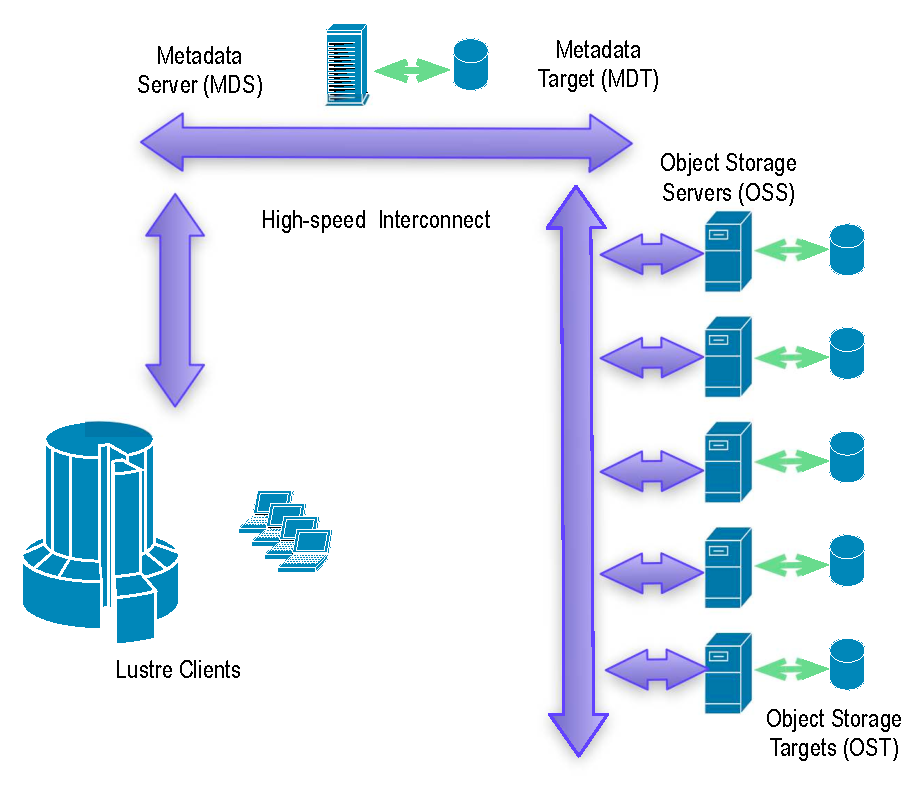
\includegraphics[scale=0.7]{img/lustre-arch}}
             \caption{Lustre components.}
             \label{fig:lustre-arch}
     \end{center}
\end{figure}

%
%At component level, Lustre system can be organized into three major pieces:
%Lustre client, Lustre server fronts (MDS/MGS, and OSS/OST) and Luster server
%backend (fsfilt and ldiskfs). In a nutshell:
%

\begin{itemize}

\item MDS (metadata servers) provides metadata services. Correspondingly, an
MDC (metadata client) is a client of those services. One MDS per filesystem
manages one metadata target (MDT). Each MDT stores file metadata, such as file
names, directory structures, and access permissions.

\item MGS (management server) serves configuration information of the Lustre
filesystem.

\item OSS (object storage server) exposes block devices and serves data.
Correspondingly, OSC (object storage client) is client of the services. Each
OSS manages one or more object storage targets (OSTs), and OSTs store file
data objects. 

\end{itemize}

The collection of MDS/MGS and OSS/OST are sometimes referred to as
\textit{Lustre server fronts}, fsfilt and ldiskfs as \textit{Luster server
backends}. In the following discussion, we start from the Lustre client side,
and follow the general data and control thread all the way to the OST and MDS.
The discussion touches on many components while skipping details to make the
structural relationship more obvious. 

\subsection*{Lustre Client}

Lustre, being a POSIX-compliant filesystem, presents a unified filesystem
interface such as open(), read(), write(), etc. to the user. In Linux, this
unified interface is achieved through Virtual File System (VFS) layer (in
BSD/Solaris, this would be known as~\url{vnode} layer). There is a shim layer
in Lustre called \textbf{llite} that is hooked with VFS to present that
interface. The file operation requests that reach llite will then go through
the whole Lustre software stack to access the Lustre filesystem, as shown in
Figure~\ref{fig:lustre_components}.

\begin{figure}[htb]
\centering
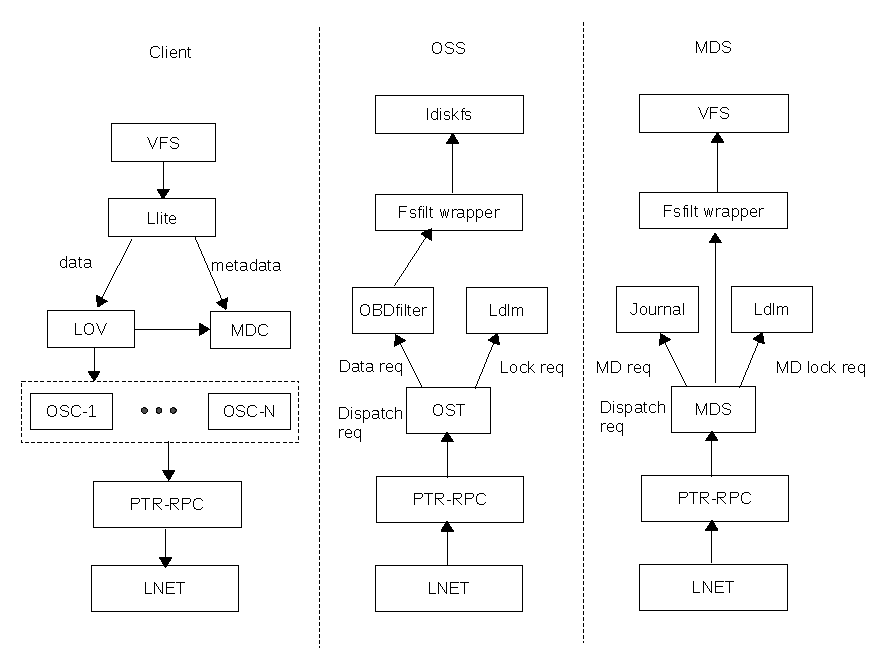
\includegraphics[width=4.5in]{img/lustre_components}
\caption{A component view of Lustre architecture.}
\label{fig:lustre_components}     
\end{figure}
 
In Lustre, general file operations such as create, open, read, etc. require
metadata information stored on \textbf{MDS}. This service is accessed through
a client interface module, known as \textbf{MDC}.

From the MDS point of view, each file is composed of multiple data objects striped
on one or more OSTs. A file object's layout information is defined in the
extended attribute (EA) of the inode. Essentially, EA describes the mapping
between file object id and its corresponding OSTs. This information is also
known as \textit{striping EA}.

For example, if file A has a stripe count of three , then its EA might look like:

\begin{Verbatim}
    EA ---> <obj id x, ost p>
            <obj id y, ost q>
            <obj id z, ost r>
            stripe size and stripe width
\end{Verbatim}

So if the stripe size is 1MB, then this would means that [0,1M), [4M,5M) ... are
stored as object $x$, which is on OST $p$; [1M, 2M), [5M, 6M) ... are stored as
object y, which is on OST $q$; [2M,3M), [6M, 7M) ... are stored as object $z$,
which is on OST $r$.

Before reading the file, client will query the \textbf{MDS} via MDC and be
informed that it should talk to \url{<ost p, ost q, ost r>} for this
operation.  This information is structured in so-called LSM, and client side
\textbf{LOV} (logical object volume) is to interpret this information so
client can send requests to OSTs.  Here again, the client communicates with OST
through a client module interface known as OSC. Depending on the context, OSC
can also be used to refer to an OSS client by itself.

All client/server communications in Lustre are coded as an RPC request and
response.  Within the Lustre source, this middle layer is known as Portal RPC, or
\textbf{ptl-rpc}: It translates and interprets filesystem requests to and
from the equivalent form of RPC request and response, and the \textbf{LNET} module to
finally put that down onto the wire.

\subsection*{OSS}

At the bottom of the OSS stack, are the familiar LNET and Portal-RPC
layers. As with the client side stack, Portal RPC will interpret the request.  The
important thing to bear in mind is that the requests handled by OSS are data
requests \footnote{As well as some size requests, such as glimpse requests from a
client}, not metadata requests. Metadata requests should be passed on and
handled by MDS stack, as shown at the rightmost column in
Figure~\ref{fig:lustre_components}.

Going up on the stack, \textbf{OST} acts like a dispatcher: it invokes
different functions based on the type of request. Broadly speaking, there are
two types of request: \textit{lock} related and \textit{data} related. The
former will be passed onto \textbf{ldlm} (Lustre distributed lock manager) to
handle and the latter will go to \textbf{obdfilter}.  The obdfilter is a module
that interconnects the Lustre stack and the regular OS stack, so to speak. It
defines a generic API that translates a Lustre-specific request to the
backend filesystem-specific request, with the help another wrapper API
component called \textbf{fsfilt}. Conceptually, fsfilt is like a VFS layer, if
you register proper file operations with it, it will use the particular
filesystem as the backend; in the case of Lustre, this backend filesystem
is currently \textbf{ldiskfs}. In the future, ZFS will be supported as backend
filesystem as well, and fsfilt could probably be redesigned or replaced by a
better filesystem-agnostic middle layer.

\subsection*{MDS}

The MDS software stack is similar to the OSS stack but, there are some
differences between them. The main difference is that the MDS software stack
does not have an obdfilter as can be seen in Figure
\ref{fig:lustre_components}. The dispatcher is called~\textbf{MDS}. Of course,
it does more than just dispatch, and it will be explained in detail in Section
\ref{sec:lustre-mdc}. For a metadata change request, MDS will do journaling a
bit differently: it will start a transaction before directly invoking the VFS
API. The particular component block may be called \textbf{dcache} as it mostly
concerns operating on a \textbf{dentry} cache, but in a larger framework, it is
really part of the VFS.



%\section{LDLM: Lock Manager}

The basic design idea of Lustre Lock Manager comes from VAX DLM. There
are some fundamental concepts we need to explain before we can dive into
the code and understand how it works.

\subsection{Namespace}

The first concept we will cover is the \textit{namespace}. Whenever you request a
lock, you are asking a lock for a certain resource in a namespace, and there is
one namespace defined per Lustre service.  To put this in a practical context,
say your Lustre system is composed of ten OSTs, then from LDLM point of view,
there are ten namespaces.  Furthermore, MDS and MGS each have their own
namespaces here. A namespace in Lustre is defined by struct
\url{ldlm_namespace}. It has a reasonable amount of comments for the fields in the
source code, so here we just focus on a few of the less-obvious ones.

\begin{figure}[htb]
\centering
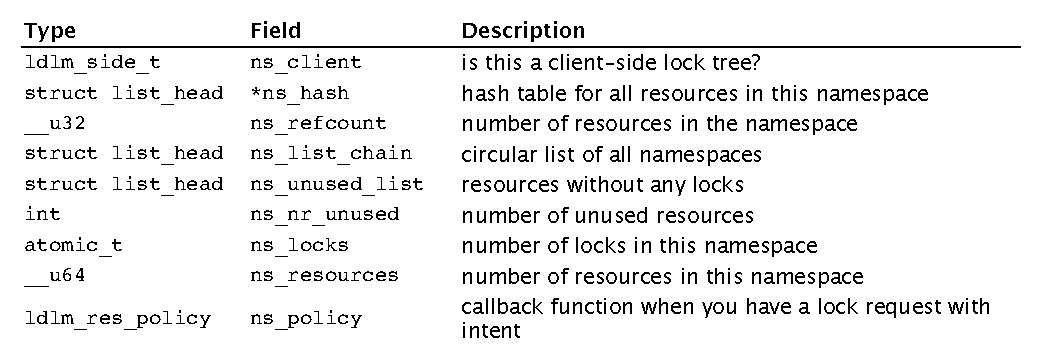
\includegraphics[width=5in]{img/lustre_ns}
\caption{The fields of \textit{ldlm\_namespace} data structure.}
\label{fig:ns}
\end{figure}

Some additional notes on \url{ns_client}: Each client only needs access to
some portions of a namespace, but not all of them. So each client carries a
so-called \textit{shadow namespace}.  \url{ns_client} is a flag that says this
namespace is for client only and is not complete (see Figure~\ref{fig:shadow} for an
illustration). \url{ns_hash} is a hash table for all resources in this
namespace. Notice that this is a pointer to the linked list, not just the
linked list itself.

\begin{figure}[htb]
\centering
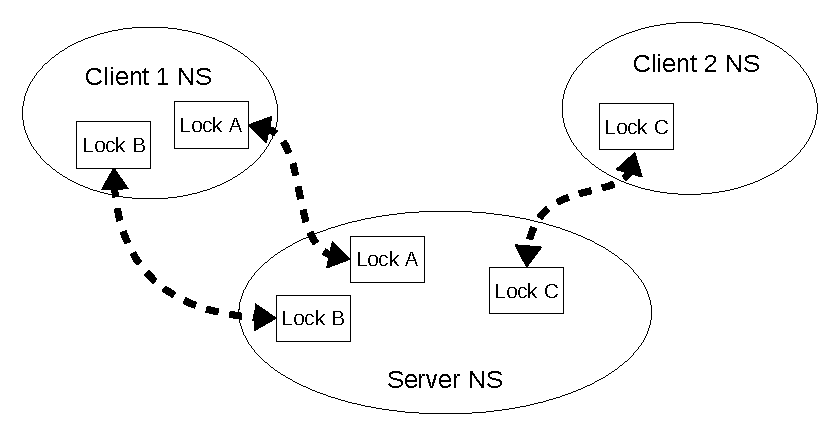
\includegraphics[width=3.5in]{img/lustre_nsclient}
\caption{Shadow namespaces on clients.}
\label{fig:shadow}
\end{figure}

\subsection{Resource}

A lock is for protecting resources. In Lustre, the most common type of
resources are files. A \textbf{local lock} refers to a lock that is private,
known only to the local entity. Correspondingly, a \textbf{global lock} is
visible to the others.  Note that ``global'' in this case may be a misnomer
-- it doesn't mean the lock is actually broadcast and known by all parties.
In Lustre, it means you have a client copy of the lock, but server also got a
copy through client request.\footnote{The lock on the server may be called 
the master lock.}

A resource is defined in struct \url{ldml_resource}. Some highlights of the
struct are discussed below.

\begin{description}

\item[\url{struct ldlm_namespace *lr_namespace}]

Points back to the namespace this resource belongs to. If the resource
is a object id (oid), then its namespace is the associated OST. If it is fid,
then its namespace is defined by the MDS.

\item[\url{struct list_head lr_granted, lr_converting, lr_waiting}]

There are three lists defined here to categorize different locks and their
states requested on this resource. \textit{Granted list} is for all locks that
have been granted use on this resource. \textit{Waiting list} is for locks
requesting the resource, but must wait due to a conflict.  \textit{Converting
list} is for locks changing mode. 

\item[\url{struct ldlm_res_id lr_name}] 

The name of the resource is defined in a struct, which is a 4$\times$64 bits long
identifier.  All types of resources, either fid or oid, will be converted to
this format as their generic resource name.

\end{description}


\subsection{Lock Type and Mode}

A lock has both a type and a mode. We discuss the mode first. There are
six lock modes along with a compatibility matrix to indicate if two
locks are compatible. The six modes are given below.

\begin{itemize}

\item \url{EX} \textbf{Exclusive mode} Before a new file is created, MDS
requests \url{EX} lock on the parent.

\item \url{PW}  \textbf{Protective Write (normal write) mode} When a client
requests a  write lock from an OST, a lock with PW mode will be issued.

\item \url{PR}  \textbf{Protective Read (normal read) mode} When a client
requests a read from an OST, a lock with \url{PR} mode will be issued. Also, if
the client opens a file for execution, it is granted a lock with \url{PR} mode.

\item \url{CW}  \textbf{Concurrent Write mode} The type of lock that the MDS
grants if a client requests a write lock during a file open operation.

\item \url{CR}  \textbf{Concurrent Read mode} When a client performs a path
lookup, MDS grants \url{inodebit} lock with the \url{CR} mode on the
intermediate path component.

\item \url{NL}  \textbf{Null mode}.

\end{itemize}

The corresponding matrix is given in Figure \ref{fig:matrix}.

\begin{figure}[htb]
\centering
\begin{Verbatim}
                                 NL  CR  CW  PR  PW  EX
                             -----------------------------
                            NL    1   1   1   1   1   1
                            -----------------------------
                            CR    1   1   1   1   1   0 
                            -----------------------------
                            CW    1   1   1   0   0   0  
                            -----------------------------
                            PR    1   1   0   1   0   0
                            -----------------------------
                            PW    1   1   0   0   0   0 
                            -----------------------------
                            EX    1   0   0   0   0   0 
                            -----------------------------
\end{Verbatim}
\caption{Lock compatibility matrix.}
\label{fig:matrix}
\end{figure}

In Lustre, four types of locks are defined, and it is up to the client to decide
what type of lock it requests.  The component that requests a lock from the
lock manager is the client, and it can be Lustre Lite, OSC or MDC. These four
types of locks are given below. 

\begin{description}

\item[\textit{extent lock}] for protecting OST data, defined by struct
\url{ldlm_extent}.

\item[\textit{flock}] for supporting a user space request on flock, defined by
struct \url{ldlm_flock}.

\item[\textit{inode bit lock}] for protecting metadata attributes, defined by
struct \url{ldlm_inodebits}.

\item[\textit{plain lock}] defined, but not in use and can be ignored.

\end{description}

\subsection{Callbacks}

Another concept associated with the lock request is the \textit{callback
function}. When a lock is created, a client can supply three type of callbacks:

\begin{description}

\item[\textit{blocking callback}] There are two conditions where this callback
will be invoked. First, if a client requests a lock conflicting with this one
(even if the request comes from the same client), then this callback is invoked,
so that if this client plays ``nice'' and has no use for this lock anymore, it
can release the lock and let the other party have it. The second case is when a
lock is revoked (after all references went away and the lock was cancelled).

\item[\textit{completion callback}] There are also two cases in which this callback will
be invoked: first, if the lock requested is granted; second, if the lock is
converted, for example, to a different mode.

\item[\textit{glimpse callback}] This callback is used to provide certain
information about underlying properties without actually releasing the lock.
For example, an OST can provide such a callback to provide information on file
size since only the OSTs know exactly the size of a file object. This callback
is then associated with the extent lock on the file object and is invoked by
the server upon receiving the client request.

\end{description}


\subsection{Intent}

An intent is a piece of data supplied with a lock enqueue indicating special
processing is needed during lock enqueue, and the data themselves are the parameters
for that processing. Namespaces can have different \textit{intent handlers}
defined for such processing.

The intent feature allows the caller of~\url{namei} and lookup to pass some information
about what they want to accomplish in the end. The net effect of this is a
reduced number of RPC requests when interacting with the MDS.

A intent is defined as follows (\url{inode.h}):

\begin{Verbatim}
struct intent {
    unsigned    int_opmask;
    void        * int_arg1;
    void        * int_arg2;
};
\end{Verbatim}

Six intention operations are defined (encoded in \url{int_opmask}). These
are get attributes, set attributes, insert or delete, open, create, and
read links.

\subsection{Lock Manager}

Now let's provide a general description of how the locking algorithm
(implemented by the lock manager) works in Lustre.  The entry call to Lustre
Distributed Lock Manager (LDLM) changes with different Lustre versions; we take
1.6 branch code as our reference. There are two major types of requests an
LDLM can service: first, when a lock is requested, and second, when a lock is
cancelled. We describe the two cases separately.

\subsubsection{Requesting a Lock}
\label{sec:requestlock}

\begin{enumerate}

\item A locking service client, whether it is a Lustre client, MDS, or OST,
usually starts with a call to \url{ldlm_cli_enqueue()}. This function first
examines if the lock requested belongs to the local namespace by checking the
flag \url{ns_client} in the namespace struct.  Remember that each LDLM instance
defines its own namespace.  If it is local, meaning that we don't have to send
RPC to communicate, we skip to step \ref{lm:local}; otherwise, we continue
processing the lock remotely.

\item If the lock request is for a non-local namespace, we need to send
\textit{lock enqueue RPC} to LDLM running on the server; this is done inside
the \url{ldlm_cli_enqueue()}. On the server side, \url{ldlm_handle_enqueue()}
unpacks the lock request first, then creates a lock (\url{ldlm_lock_create()}).
This lock is just an initial one with some fields filled in from the original
lock request; it has not been granted yet. You can determine if a lock is
granted or not by checking:

    \begin{Verbatim}
    if (lock->req_mode == lock->granted_mode) {   /* granted */
        ...
    }
    \end{Verbatim}

Now we move to the next step to check if the lock can be granted and what lock
should be granted.

\item \url{ldlm_lock_enqueue()} is the core step for granting the lock. It
checks if the lock intent is set. If no intent is set, then it checks for the
lock type and invokes the policy function defined for this lock type. The
policy function will determine if the request lock can be granted or not. 

If the lock intent is set, go to step \ref{lm:intent}.

\item For the resource for which the lock is being requested, two conditions
need to be checked as given below.
  
  \begin{itemize}
  \item Are there any conflicts with those granted locks?
  \item Are there any conflicts with those waiting locks?
  \end{itemize}

If the answer to both questions is no, then no conflict is found, and the lock can be granted.
Call \textit{completion AST}\footnote{AST is the acronym for Asynchronous System
Trap from VMS lock design. Here, we consider it to be synonymous with a
callback.}, return the granted lock, and we are done.  Otherwise, continue.

\item For each conflicting lock, we need to call \textit{blocking AST}.
Blocking AST checks if the lock is held at the server, then just sets a flag. If
the lock is held at the client, then a \textit{blocking RPC} request must be
sent. Either way, after all these are done, put this new lock request on the
waiting list, then return the lock with status as being blocked.

A more detailed policy function implementation is provided later.

\item \label{lm:intent} If the lock intent is set, then all that needs to be done is to
invoke the intent handler. The key point is that LDLM does not interpret intents. The
parties communicating with each other with intent do that; for example, MDS needs to
register its intent handler, and OST needs to register its intent handler. In general,
intent handler is registered per namespace by calling
\url{ldlm_register_intent()}. It is the LDLM's responsibility to invoke them.
The intent handler will determine if the lock can be granted or not. LDLM just
returns the result of their verdict.

\item \label{lm:local} For a local lock request, it goes to a different branch
at \url{ldlm_cli_enqueue_local()}, except that in this case it doesn't need to
send an RPC anymore. It will need to go through the two phases described above:
creating a lock first, then calling \url{ldlm_lock_enqueue()} to check if this
can be granted. If either lock is granted or if there are any errors, it
returns immediately with the lock marked correspondingly. Otherwise, lock request
is being blocked, and it needs to wait for it.

Please note that a server (e.g., MDS or OST) can initiate a lock request by
directly calling \url{ldlm_cli_enqueue_local()} since they know the lock must
be held by the local LDLM server. 

\end{enumerate}

\subsubsection{Canceling a Lock}

A lock is usually released involuntarily, and the owner will hold it as long as
possible until: someone is asking for a conflicting lock, LDLM sends out
a blocking AST, and the block AST handler invoked on the LDLM client side. Now we enter
the canceling process.  There are three counters in the lock that are related
to the cancelling process. These can be listed as (1) counts of active
readers, (2) counts of active writers, and (3) counts of users.

\begin{enumerate}

\item The entry point for cancelling a lock is \url{ldlm_cli_cancel()}. This
function first checks if the sum of active readers and writers is zero. If not,
it means another process on the same client is using the lock so, we do
nothing.  Eventually, the other client(s) will release the lock and follow the
same code path and reach this checkpoint, then it will move to the next
step.

\item Now when the sum of readers and writes count reaches zero, we call blocking
AST with a flag set indicating this lock is being revoked. 

\item Check if this lock is in the local namespace. If it is not, send
\textit{cancel RPC} to client (Lustre client). If so, the server side calls
\url{ldlm_handle_cancel()} to cancel the lock.

A cancel operation essentially involves steps that take this lock of all the
lists it is currently on, such as granted list, waiting list, etc. Later,
\url{obd_cancel()} will be called not to cancel the lock, but just to release
the references on reader and writer counts.

\item Now that the lock has been cancelled, server can reprocess all waiting locks
on the resource. It essentially goes through the same logic to determine if
their lock requests can be granted.

\item If a waiting lock request can be granted, move it to the granted lock
list, then invoke the \textit{completion AST}.

\end{enumerate}

\subsubsection{Policy Function}

As we discuss in the section on requesting a lock (\ref{sec:requestlock}),
policy function is being called to determine if the requested lock is in
conflict with existing requests, based on the lock type. We have four lock
types, and these are \textit{inodebits}, \textit{extent}, \textit{flock}, and
\textit{plain}. Therefore, we need four policy functions. They all follow a
similar overall flow, with some minor changes.  In this section, we give
an overall description on the overall flow.

\begin{enumerate}

\item There are two given parameters and these are lock request and a flag of
\url{first_enq}. This flag means to signal if this is first time we do an
enqueue request. If this is the first time, the waiting list needs to be processed
and send blocking ASTs when necessary. If this is not the first time, then we
already sent out blocking AST before, so there is no need to do it again.

Another important thing about \url{first_enq} parameter is that when it is not set
(which means we are reprocessing a lock already in the waiting list),
we stop processing the waiting list after we find our own earlier entry in the
list. Since the rest of the locks were enqueued at a later point in time, those
can be ignored safely.


\item \label{lm:helper} The policy function calls on a helper function for
real work, passing in as parameters both lock list, enqueue flag, as well as a
RPC list, either \url{NULL} or a empty list. The first time, the helper
function is called with a granted lock list. For each lock in the list, it
performs the following conflict detection.\footnote{An implementation can
choose to implement its own policy function and conflict detection, not
necessarily follow exactly as we presented here.}

  \begin{enumerate}

  \item It always starts with mode checking. If two locks are compatible (refer
  	to the previous section for the compatibility matrix), then no more checking is
  	needed, and a lock can be granted. We continue only if locks are incompatible and the lock
  	type is not \textbf{plain} since plain lock is not actually in use.

  \item For the \textbf{extent} lock type, if the interval or range does not 
  	intersect, then there is no conflict. However, within the boundary of a stripe 
	size, LDLM always tries to grant the largest extent possible to reduce the 
	possibility of further requests in case the client asks for more locks.

  \item For the \textbf{inodebits} lock type, if the bits requested (Lustre has a
	64-bit lock space, but only 3 are being used) intersect, then there are
	conflicts.  \footnote{It groups locks based on the bits (more precisely, it is
	based on the integers formed by the 3-bit value since only 3-bits are in use),
	so you only need to check one member in each group to make a decision, as a
	performance optimization.}

  \end{enumerate}

If the RPC list is \url{NULL}, we stop and return right after the first
conflict is detected, since by passing \url{NULL}, we obtained all the
information that the caller requires. 

If the RPC list is not \url{NULL}, we need to continue for each remaining locks
and add the conflicting lock into the RPC list.


\item If no conflicts are found, then the lock is granted. Otherwise, for each
conflict lock in the RPC list, we invoke blocking AST.


\item If first enqueue flag is set, then we go back to step \ref{lm:helper},
but this time, we invoke the helper function with the lock list set as waiting list
instead of granted list.


\end{enumerate}


\subsection{Use Cases}

In this section, we use examples to give high level overview on
processing lock requests.

\subsubsection*{MDS: One Client Read}

Let's assume client $C_1$ wants to open the file \url{/d1/d2/foo.txt} to read.
During the VFS path lookup, Lustre specific lookup routine will be invoked (see the
Lustre Lite section for details on this). The first RPC request is lock enqueue
with lookup intent. This is sent to MDS for lock on \url{d1}. The second RPC
request is also lock enqueue with lookup intent and is sent to MDS asking
inodebits lock for \url{d2}. The lock returned is an inodebits lock, and its
resources would be represented by the fid of \url{d1} and \url{d2}.

The subtle point to note is, when we request a lock, we generally need a
resource id for the lock we are requesting. However in this case, since we
don't know the resource id for \url{d1}, we actually request a lock on its
parent \url{/}, not on the \url{d1} itself. In the intent, we specify it as a
lookup intent and the name of the lookup is \url{d1}. Then, when the lock is
returned, the lock is for \url{d1}. This lock is (or can be) different from
what the client requested, and the client notices this difference and replaces
the old lock requested with the new one returned.

The third RPC request is a lock\_enqueue with open intent, but it is not asking for
lock on \url{foo.txt}.\footnote{Lustre Lite always decides no need for a lock
unless it is from NFS.} That is, you can open and read a file without a lock
from MDS since the content is provided by OST.  Requesting locks from an OST is
a different matter and is discussed later.

In other words, what happens at open is that we send a lock\_request, which
means we \textit{do} ask for a lock from LDLM server.  But, in the intent data itself, we
might (or not) set a special flag if we are actually interested in receiving
the lock back. And the intent handler then decides (based on this flag),
whether or not to return the lock.


If \url{foo.txt} exists previously, then its  fid, inode content (as in owner,
group, mode, ctime, atime, mtime, nlink, etc.) and striping information are
returned.

If client $C_1$ opens the file with the \url{O_CREAT} flag and the file doesn't
exist, the third RPC request will be sent with open and create intent, but
still there will be no lock requests. Now on the MDS side, to create a file
\url{foo.txt} under \url{d2}, MDS will request through LDLM for another
\url{EX} lock on the parent directory. Note that this is a conflicting lock
request with the previous \url{CR} lock on \url{d2}. Under normal
circumstances, a fourth RPC request (blocking AST) will go to client $C_1$ or
anyone else who may have the conflicting locks, informing the client that
someone is requesting a conflicting lock and requesting a lock cancellation.
MDS waits until it gets a cancel RPC from client. Only then does the MDS get the
\url{EX} lock it was asking for earlier and can proceed.\footnote{In the current
code, client gets smart. When it sees that it will create a new file, it cancels
the lock on \url{d2} itself by embedding the cancel operation on the third RPC
request. This saves two RPCs, one blocking AST from MDS to client and one
cancel RPC from client to MDS.}
 
If client $C_1$ opens the file with \url{LOV_DELAY} flag, MDS creates the file
as usual, but there is no striping and no objects are allocated. User will
issue an \url{ioctl} call and set the stripe information, then the MDS will
fill in the EA structure.

\subsubsection*{MDS: Two Clients}

If $C_1$ wants to create a file \url{foo.txt} under the directory \url{/d1/d2},
then no locks are required on \url{foo.txt}, but it will request a lock on
\url{d2} with the intent of instructing MDS to ``open and create" the file
\url{foo.txt} and possibly to return a lock on that file.

It acquires a \url{CW} lock intentionally on \url{foo.txt}.  Now $C_2$ comes in
and wants to create a new directory \url{d3} under \url{/d1/d2}. At this point
nothing will change as far as the \url{CW} lock is concerned.

\subsubsection*{OST: Two Clients Read and Write}

After the MDS fills in the EA structure, the client has the file handle and
stripe information. The client can now talk to OSTs. Let's assume we have four OSTs
and two clients. Client $C_1$ reads file $A$ and the second client $C_2$
writes to file $A$. We further assume that $C_1$ wants to read data objects,
$A_1$, $A_2$, $A_3$, and $A_4$.

First, client $C_1$ sends lock enqueue requests to OSTs 1 through 4 in
parallel, asking for read lock with intent flag set. What it means is, if any
of the objects client $C_1$ is asking has a blocking request, don't try to get
the lock, just return back the information (file size, modification time, etc.)
described by a data structure called \url{lvb} (Lustre Value Block) (the lock
request is a glimpse because it has intent flag set). 

If there are no conflicts, the client will be granted read locks on the
entire file objects, with lock mode as \url{PR}. Now the client has four read
locks on four OST file objects. Let's further assume that the client only wants to
read $A_1$. Since it has the lock, it can now go ahead and read it.

Assume $C_2$ is writing to OST3. Instead of returning a \url{PR} lock, OST3
will contact $C_2$ and ask for the \url{lvb} information. It then would return
this format back to $C_1$: ``I am not issuing you the lock on $A_3$, but here
is the state of that object''.

This was done just to determine the file size, and we need to know the file size,
for example, if we are trying to read beyond the file size.  If the content of
read falls into the object you already hold a \url{PR} lock on, then no further
RPCs for that lock are needed.

Now if the content the client needs to read is on $A_3$, then it has no choice
but to send a read lock request (without intent this time) to OST3.  Within the
request itself, the client should also make clear to what \textit{extent} it is
requesting the lock. If the extent it is requesting is not conflicting
(intersecting reads) with the \url{PW} write lock $C_2$ is holding, then the
read lock request will be immediately granted.

If a conflict exists, then OST3 will reply to $C_1$ that the lock request is
not granted and at the same time, it will send a blocking request to $C_2$.
There are two cases to consider from the perspective of $C_2$:

\begin{enumerate}

    \item If the \url{write()} system call is done, meaning that all data has
    been written to some buffer (maybe not to disk yet), then the buffers will
    have the dirty flag set. In that case, the client flushes all dirty buffers, probably
    through one or more bulk writes. Then it releases the lock (lock
    reference count is now zero) by sending a cancel RPC to OST3.

    \item If the \url{write()} is still in progress, then the system call
    hasn't returned yet. At this point, the lock reference count is non-zero and
    the blocking AST won't reach the lock logic.
    Only after the write system call finishes (it actually means at
    least two things here, one, the data is all in cache and two, the lock
    reference count is decreased to zero), then it can go to the step explained above.

\end{enumerate}

After OST3 gets the cancel request from $C_2$, it will send a completion
AST to client $C_1$, telling that now its lock request is granted.

We don't explain a case where both clients do read because it is trivial, as  
both of them can get \url{PR} locks, even with their extent intersecting.

If one client doesn't play nice and doesn't cooperate in releasing its lock,
then a timer is started the moment it was sent a blocking AST. If the client
doesn't release the lock and there is no ongoing I/O under that lock for the
duration of the timeout, then the client is evicted. However, if there is
ongoing I/O, then on every I/O RPC the timeout is prolonged.

\begin{comment}
the OST3 checks the last bulk write and starts the
obd timeout, when it expires without receiving another bulk write, the
client will be evicted.
\end{comment}

\begin{comment}

int flock(int fd, int operation)

- it is advisory

   - it apply to entire file

- three operations: LOCK_SH (shared), LOCK_EX (exclusive), LOCK_UN
(remove existing lock by this process)

- locks created by flock() are associated with a open file. multiple
process may point to the same lock, say when dup() is called.

- a lock is released when LOCK_UN operation is done on any of
these duplicate descriptors, or when all such descriptors have been
closed.

- A process may only hold one TYPE of lock (shared or exclusive) on a
file. Subsequent flock() call on an already locked file will convert an
existing lock to the new lock mode.



One of the first three will be part of so called policy data, defined as a
union:

    typedef union {
        struct ldlm_extent      l_extent;
        struct ldlm_flock       l_flock;
        struct ldlm_inodebits   l_inodebits;
    } ldlm_policy_data_t;




    struct list_head    l_lru;
    struct list_head    l_res_link;
    struct list_head    l_extents_list;
    struct list_head    l_cache_locks_list;
    struct list_head    l_pending_chain;
    struct hlist_node   l_exp_hash;
    struct list_head    l_bl_ast;
    struct list_head    l_bp_ast;
    struct list_head    l_sl_mode;
    struct list_head    l_sl_policy;

Q: need more explanation on struct ldlm_resource

    is there a tree here?
    
    struct list_head        lr_hash;
    struct ldlm_resource    *lr_parent;
    struct list_head        *lr_children;
    struct list_head        *lr_childof;




IMPLEMENTATION

In Lustre, the client of DLM includes MGS, OSC, and MDC. 


There are two important data structure defined for on the wire
communication. 

struct ldlm_request
struct ldlm_reply
struct ldlm_lock_desc   (when server returns the lock info, this is the
struct used)
struct ldlm_resource_desc


HOW LOCK IS CREATED?

struct ldlm_lock *ldlm_lock_create( ... )

1. get the resource through res_id: 

    res = ldlm_resource_get(ns, NULL, res_id, type, 1);

2. allocate new lock

    lock = ldlm_lock_new(res)

3. why try to release the resource?

    ldlm_resource_putref(res)

4. fill in the struct ldlm_lock such as mode, data, callback, and current
process id

5. if this is extent lock, allocate interval tree node

6. if extra data is to be passed, allocate space for it: lock->l_lvb_data;

7. return lock.


HOW REMOTE LOCK IS REQUESTED?

ldlm_error_t ldlm_lock_enqueue()

1. no idea on the first chunk of code Q:
   what is a reply lock?



\end{comment}




%\section{MDC and Lustre Metadata}
\label{sec:lustre-mdc}

\subsection{MDC Overview}

The MDC component is layered below Lustre Lite. It defines a set of
metadata related functions that Lustre Lite can call to send metadata requests
to MDS.  The set of functions is implemented in \url{lustre/mdc}, and we 
discuss them in Section \ref{sec:stripingapi}.

Lustre Lite passes the request parameters in a \url{mdc_op_data} data
structure, and all requests must eventually be converted to a structure known
as the \url{ptl_request}.  Therefore, before a RPC request can be carried out,
there are several steps for preparing it (\textit{packing}). Within the
\url{mdc_lib.c}, there are a number of functions defined for this purpose. In
turn, some of these functions actually invoke packing helper methods provided
by the Portal RPC layer.

Once \url{ptl_request} is ready, MDC can then invoke \url{ptlrpc_queue_wait()}
to send the request.  This is a synchronous operation, and all metadata
operations with intent are also synchronous.  There are other ptlrpc methods
for send operations and used for metadata operations without intent
(\textit{mdc\_reint})---this is done in code \url{mdc_reint.c}.

For the most part, the driver of converting from \url{mdc_op_data} to
\url{ptl_request} and the call to enqueue the request are done in function
\url{mdc_enqueue}, implemented in \url{lustre/mdc/mdc_locks.c}.


\subsection{Striping EA}
\label{sec:stripingea}

Depending on where the striping EA is created or used, there are three formats:

\begin{itemize}

  \item On-disk format, used when it is stored on MDS disk, described by
\url{struct lov_mds_md}.

  \item In-memory format, used when it is read into the memory and unpacked,
described by \url{struct lov_stripe_md}.

  \item User format, used when the information is to be presented to the user,
described by \url{struct lov_user_md}.

\end{itemize}


The user format differs from on-disk format in two aspects: 

\begin{itemize}

\item The user format has \url{lmm_stripe_offset}, which on-disk format does
not have. This field is used to transfer the \url{striping_index} parameter to
Lustre when user wants to set a stripe.

\item The user format has \url{lmm_stripe_count} as 16-bit, whereas on-disk
format has this field as 32-bit.

\end{itemize}

%\begin{figure}[htb]
%\includegraphics[width=5in]{img/struct_lov_mds_md}
%\end{figure}


\subsection{Striping API}
\label{sec:stripingapi}

Five types of APIs are defined to handle striping EA. These are listed below.

\begin{description}

  \item[set/get API] To set or get a stripe EA from storage. It operates
  on on-disk striping EA.

  \begin{Verbatim}
  int fsfilt_set_md(struct obd_device *obd, struct inode *inode, 
                 void *handle, void* md, int size, const char *name)
  int fsfilt_get_md(struct obd_device *obd, struct inode *inode, 
                 void *md, int size, const char *name)            
  \end{Verbatim}

  Here, \url{md} is the buffer for the striping EA, \url{handle} is the journal
  handle, and \url{inode} refers to the MDS object.
  
  \item[pack/unpack API] As striping EAs are stored in packed format on disk, they
   are unpacked after \url{fsfilt_get_md()} is called. These APIs can be
   used for both on-disk and in-memory striping EA. 
  
  \begin{Verbatim}
  int obd_packmd(struct obd_export *exp, struct lov_mds_md **disk_tgt,
                 struct lov_stripe_md *mem_src)
  int obd_unpackmd(struct obd_export *exp, struct lov_stripe_md **mem_tgt,
                  struct lov_mds_md *disk_src, int disk_len)
  \end{Verbatim}
  
  Here, \url{mem_src} points to the in-memory structure of striping EA, and \url{disk_tgt}
  points to the disk structure of striping EA. Conversely, \url{disk_src} is the source
  for on-disk striping EA, while \url{mem_tgt} is the  target for in-memory
  striping EA.
  
  \item[alloc/free API] Allocates and frees striping EA in memory and on-disk. 
  \begin{Verbatim}
  void obd_size_diskmd(struct obd_export *exp, struct lov_mds_md *dis_tgt)
  int obd_alloc_diskmd(struct obd_export *exp, struct lov_mds_md **disk_tgt)
  int obd_free_diskmd(struct obd_export *exp, struct lov_mds_md **disk_tgt)
  int obd_alloc_memmd(struct obd_export *exp, struct lov_stripe_md **mem_tgt)
  int obd_free_memmd(struct obd_export *exp, struct lov_stripe_md **mem_tgt)
  \end{Verbatim}
  
  \item[striping location API] Returns data object location information from striping EA.
  
  \begin{Verbatim}
  obd_size love_stripe_size(struct lov_stripe_md *lsm, obd_size ost_size, int stripeno)
  int lov_stripe_offset(struct lov_stripe_md *lsm, obd_off lov_off, 
                     int stripeno, obd_off *obd_off)  
  int lov_stripe_number(struct lov_stripe_md *lsm, obd_off lov_off)
  \end{Verbatim}

  Here, \url{lov_off} is the file logical offset. The \url{stripeno} is the stripe number
  of the data object. 

  \item[lfs API] User-level API to handle striping EA and is used by the \url{lfs}
  utility.

  \begin{Verbatim}
   int llapi_file_get_stripe(const char *path, struct lov_user_md *lum)
   int llapi_file_open(const char *name, int flags, int mode, 
      unsigned long stripe_size, int stripe_offset, int stripe_count,int stripe_pattern)
   \end{Verbatim} 

    Here, \url{llapi_file_get_stripe()} will return a user striping EA given a path, and
    \url{llapi_file_open()} opens/creates a file with a user specified stripe
    pattern. It is also worth noting that \url{stripe_offset} is the same as
    \url{stripe_index} used in user space, and it is the OST index of the first
    stripe.
    
\end{description}



%\section{Portal RPC}

Portal RPC provides basic mechanisms for

\begin{itemize}

  \item sending requests through imports and receiving replies,

  \item receiving and processing requests through exports and sending replies,

  \item performing bulk data transfer, and

  \item error recovery.

\end{itemize}

\subsection{Client Side Interface}

We will first discuss the interface of Portal RPC without going into
implementation details. We will use the LDLM's send mechanism as an example.
For this example, LDLM is sending a blocking AST RPC to a client that is
the owner of a given lock (\url{ldlm_server_blocking_ast}) and also acting as
the lock manager. This example will help us better illustrate how a client uses
Portal RPC API.  

First, we prepare the size for this request as given below.

\begin{Verbatim}
struct ldlm_request *req;
__u32 size[] = { [MSG_PTLRPC_BODY_OFF] = sizeof(struct ptlrpc_body),
    [DLM_LOCKREQ_OFF] = sizeof (*body) };
\end{Verbatim}

A request can be seen as a sequence of records, where the first record has an
offset of 0, the second record has an offset value 1, and so on. Once the size
is determined, we can invoke \url{ptlrpc_prep_req()}. The prototype of this
function is as follows:

\begin{Verbatim}
struct ptlrpc_request *
  ptlrpc_prep_req(struct obd_import *imp, __u32 version, int opcode, 
                int count, __u32 *lengths, char **bufs)
\end{Verbatim}

The RPC communication needs an import on the client's side, and it is created
during the connect phase. The \url{*imp} points to this particular import, and
\url{version} specifies the version to be used by the Portal RPC internals to
pack the data. Packing here is the  on-the-wire format that defines how the
buffers are actually situated in the network packet. Each subsystem defines a
version number to distinguish its layout request---for example, MDC and MDS
define their version, MGC and MGS define another. 

The \url{opcode} specifies what this request is about. Each subsystem defines
a set of operation codes (see \url{lustre_idl.h} for more information).
The \url{count} is the number of buffers needed for this request, and
\url{*length} is an array with each element specifying the size of the
corresponding requested buffer.  The final parameter signals Portal RPC to
accept (copy the data over) and process the incoming packet as is.  For our
example, this function is invoked as given below.

\begin{Verbatim}
req = ptlrpc_prep_req(lock->l_export->exp_imp_reverse,
    LUSTRE_DLM_VERSION, LDLM_BL_CALLBACK, 2, size, NULL);
\end{Verbatim}

This declaration indicates that there are two buffers requested and the size of
each buffer is represented by \url{size} in the parameter list.

In addition to the housekeeping, the above call allocates the request buffer and
saves it in  \url{req->rq_reqmsg}.  The address of the interested record can be
acquired by specifying the record offset:

\begin{Verbatim}
body = lustre_msg_buf(req->rq_reqmsg, DLM_LOCKREQ_OFF, sizeof(*body)); 
\end{Verbatim}

On the server side, we see this same helper method with similar input parameters
used to extract the field of interest. Once the buffer structure is obtained,
necessary fields for the request can be further filled in. After all is done,
there are several ways to send the request, as listed here.

\begin{description}

\item[\url{ptl_send_rpc()}] A primitive form of RPC sending, which doesn't wait
for a reply and doesn't try to resend when failure occurs. It is not a preferred
way of doing RPC send.

\item[\url{ptlrpcd_add_req()}] A completely asynchronous RPC sending, handled
by the ptlrpcd daemon.

\item[\url{ptlrpc_set_wait()}] A synchronous RPC sending of multiple messages,
which returns only when it gets if all of the replies back. First,
\url{ptlrpc_set_add_req()} must be used to add the request to a pre-initialized
set, which contains one or more requests that must be sent together. 

\item[\url{ptlrpc_queue_wait()}] Probably the most common way of sending RPC,
which is synchronous and returns only after an RPC request is sent and a reply is
received.

\end{description}

The last step after invoking this RPC request is to release the resource
references by calling \url{ptlrpc_req_finished(req)}.

\subsection{Server Side Interface}

The server side uses Portal RPC in a completly different way from the
client side. First, it initializes the service with the function call given
below.

\begin{Verbatim}
struct ptlrpc_service * ptlrpc_init_svc (
    int nbufs,             /* num of buffers to allocate */
    int bufsize,           /* size of above requested buffer */ 
    int max_req_size,      /* max request size server will accept */
    int max_reply_size,    /* max reply size server will send */ 
    int req_portal,        /* req service port in lnet */
    int rep_portal,        /* rep service port in lnet */
    int watchdog_factor,   /* wait time for handler to finish */
    svc_handler_t handler, /* service handler function */
    char *name,            /* service name */
    cfs_proc_dir_entry_t *proc_entry, /* for procfs */
    svcreq_printfn_t svcreq_printfn,  /* for procfs */
    int min_threads,        /* min # of threads to start */
    int max_threads,        /* max # of threads to start */
    char *threadname        /* thread name prefix */
)
\end{Verbatim}

Once the call returns, the request can come in and the registered handler
function will be called. Usually, server divides the task at hand into several
types. For each type, it creates a different pool of threads. These threads
could share the same handler. The reason for different pools is to prevent
starvation. In some cases, multiple pools also prevent deadlocks, where all
threads are waiting for some resource to become free to handle a new RPC. 

\subsection{Bulk Transfer}
\label{sec:bulktransfer}

The client first sends a bulk RPC request. Let's assume this is a write request.
It contains descriptions of what to send. Now the server processes the request,
allocates the space, and then takes control of the data transfer. The next
RPC from the server will perform a bulk transfer of the data to the
pre-allocated spaces. One such example is done in the
\url{osc_brw_pre_request()}. Let's walk through the process: 

\begin{enumerate}

\item Bulk transfer is initiated with the preparation as discussed before.
However, the prepare request is different in the sense that we are asking the
request from a pre-allocated pool, which is the case if the request itself can be
associated with a low-memory situation.

\begin{Verbatim}
req = ptlrpc_pre_req_pool(cli->cl_import, LUSTRE_OST_VERSION, 
                                  opc, 4, size, null, pool)
\end{Verbatim}

The \url{opc} in this case can be, for example, \url{OST_WRITE}.

\item Next, we specify the service portal. In the import structure, there is a
default portal that this request will go, but in this case for the sake of the
example, let's assume the request will be handled by a specific portal:

\begin{Verbatim}
req->rq_request_portal = OST_IO_PORTAL;
\end{Verbatim}

\item Then, we need to prepare the bulk request. We pass in as parameters the
pointer to the request, number of pages, type, and destination portal. The
return is a bulk descriptor for this request. Notice that the bulk request goes
to a different portal:

\begin{Verbatim}
struct ptlrpc_bulk_desc desc = ptlrpc_prep_bulk_imp(req, page_count, 
             BULK_GET_SOURCE, OST_BULK_PORTAL);
\end{Verbatim}

\item For each page to be transferred, we invoke the
\url{ptlrpc_prep_bulk_page()} and add one page at time to the bulk descriptor.
There is a flag in the request indicating that this is a bulk request and we
should check this descriptor to obtain all the layout information on pages.

\begin{Verbatim}
struct ptlrpc_request {
    ...
    struct ptlrpc_bulk_desc *rq_bulk;
    ...
}
\end{Verbatim}

\end{enumerate}

At the server side, the overall preparation structure is similar, but instead
of preparing for import, now it prepares for an export. An example of it can be
seen in \url{ost_brw_read()} in ost handler.

\begin{Verbatim}
desc = ptlrpc_prep_bulk_exp(req, npages, BULK_PUT_SOURCE, OST_BULK_PORTAL);
\end{Verbatim}

The server side also needs to prepare each bulk page. Later, the server side
can start the transfer by:

\begin{Verbatim}
rc = ptlrpc_start_bulk_transfer(desc);
\end{Verbatim}

At this point in time, the first RPC request from the client has been
processed by the server, and the server is ready for the bulk data transfer.
Now the server can start the bulk RPC transfer as we mentioned at the
begining of this section.

\subsubsection*{NRS Optimization}

On the server side, another point to note is that we can receive a huge number
of descriptors that describe the page layout to read or write. This presents an
opportunity for an optimization if there are any neighboring reads or writes
going to the same region. If there are, perhaps they can be grouped and
processed together. That is the subject of the Network Request Scheduler
(NRS). This also displays the significance of a two-phase bulk transfer, which
allows us to get an idea of the incoming/outgoing data without actually getting the
data first, so that they can be reorganized for better performance. The second
reason for the two-phase operation is that as the service initialization
increases on the server, a certain amount of buffer space is allocated. When
client requests come in, they will be buffered in this space first before further
processing, as pre-allocating a huge amount of space there just to accommodate
potential bulk transfers is not preferred. Also, it is important not to overwhelm
server buffer space with big data chunks, and two-phase operation helps in that
context as well.

\subsection{Error Recovery: A Client Perspective}

Most of the recovery mechanism is implemented at the Portal RPC layer.  We
start with a portal PRC request which is passed down from the upper level.
Inside Portal RPC, there are two lists maintained by the import that are
important to our discussion. These are the \textit{sending} and \textit{replay}
lists. The import also maintains \url{imp->states} and \url{imp->flags}. The
possible states are \textit{full}, \textit{connecting}, \textit{disconnecting},
and \textit{recovery}, and flags can be \textit{invalid}, \textit{active} and
\textit{inactive}. 

After the health status of the import is checked, the send request will
continue. The sequence of the steps is outlined here:

\begin{enumerate}

\item Send the RPC request, then save it into the sending list. Also start
the \textbf{obd timer} at the client side.

\item If a server reply is received before the timeout expires and the request is
\textit{replayable}\footnote{Replay request only refers to those that will
modify the on-disk data. For example, read is not a replayable request, but
during recovery, they can still be resent if they are in the sending list.},
then unlink it from the sending list and link it to the replay list. If the
request is not replayable, then upon receiving the reply, remove the request
from the sending list.

A reply from the server doesn't necessarily mean it committed the data to the
disk (assuming the request alters on-disk data).  Therefore, we must wait for a
transaction commit (a transaction num) from the server, which means that the
change is now safely committed to the disk.  This last server-committed
transaction number is usually piggybacked with every server reply.  

Usually, a request from MDC to MDS is replayable, but an OSC to OST request is
not, and this is only true if the asynchronous journal update is not enabled.
There are two reasons:

  \begin{itemize}
  
  \item First, a data request (read or write) from OSC to OST can be very
  large, and keeping them in memory for replay can be a huge burden
  on memory.

  \item Second, OST uses only direct I/O (at least for now). The reply itself,
  along with transaction number, is enough of a guarantee to say the commit is
  done.

  \end{itemize}

\item If a timer expires, then client marks this import state from \textit{full}
to \textit{disconnect}. Now the pinger kicks in and if the server responds to
the pinger, then the client will try to reconnect (connect with reconnect
flags). 

\item If the reconnect is successful, then we start the recovery process. We
now mark the state as \textit{recovery} and start sending the requests in the
replay list first, followed by the requests in the sending list.

\end{enumerate}

The key point about the pinger is that if requests are being sent frequently enough, 
then the pinger is not needed. It is activated only if a client 
has an extended idle period, and the pinger is used to keep the
connection alive with the server so that it will not get evicted due to
inactivity. On the other hand, if client went offline for whatever reason,
the server will not get pinged by the client, and the server can still evict this
client.



%\section{OST and obdfilter}
\label{sec:ost-and-obdfilter}

\begin{quote}
\begin{Verbatim}
/* Sigh - really, this is an OSS, the _server_, not the _target_ */
static int ost_setup(struct obd_device *obd, obd_count len, void *buf)
{ ... }
\end{Verbatim}
\begin{flushright}
\textit{\small from Lustre source tree b16}
\end{flushright}
\end{quote}

Lustre source tree \url{lustre/ost} and all function names prefixed with
\url{ost_} should probably be regarded as server (OSS) functions, if we
understand the above comment correctly.

\subsection{OSS as OST}

OST is loaded as a kernel module. It works closely with obdfilter and does most
of the server/OST side of the work. Between these two layers, OSS is the switch
layer or the \textit{thin} layer, and it interprets requests from Portal RPC,
prepares for requests, and then passes requests to obdfilter for further
processing. In the following discussion, we focus on two aspects of it: initial
setup and switching structure, implemented by \url{ost_setup()} and
\url{ost_handle()}, respectively.

\subsubsection*{Initial Setup}

\begin{itemize}

\item First, the OST checks if the OSS thread number is specified. If not, then it
computes the minimum number of threads based upon the CPU and memory and
ensures that there is 4x dynamic range between the minimum and maximum number
of threads. 
\begin{Verbatim}
    oss_min_threads = num_possible_cpus() * num_physpages >> (27 - CFS_PAGE_SHIFT);
    if (oss_min_threads < OSS_THREADS_MIN)
         oss_min_threads = OSS_THREADS_MIN;
    /* Insure a 4x range for dynamic threads */
    if (oss_min_threads > OSS_THREADS_MAX / 4)
         oss_min_threads = OSS_THREADS_MAX / 4;
    oss_max_threads = min(OSS_THREADS_MAX, oss_min_threads * 4 + 1);
\end{Verbatim}


To get the obd device of the OST; the following function call is used.

\begin{Verbatim}
struct ost_obd *ost = &obd->u.ost;
\end{Verbatim}

\item Then, the server side initiates RPC services by:
\begin{Verbatim}
ost->ost_service = ptlrpc_init_svc( , , , , , , ost_handle, , , , "ll_ost");
\end{Verbatim}

The function returns the pointer to struct \url{ptlrpc_service}. One important
thing to note is that we have supplied a handler, \url{ost_handle}.  Once the
service is set up as shown below, Portal RPC will dispatch the request to this
handler for further processing. That is the subject of the following
section.

\item The prtrpc threads are started as:

\begin{Verbatim}
rc = ptlrpc_start_threads(obd, ost->ost_service);
\end{Verbatim}

\item The similar call sequence is repeated for creating \textit{ost create}
threads and the returned service handle is assigned to
\url{ost->ost_create_service}. It is also repeated for \textit{ost io} threads,
and a service handle is assigned to \url{ost->ost_io_service}.

\item And finally, the ping eviction service is started.

\end{itemize}

\subsubsection*{Dispatching}

The handler function takes one input parameter, \url{struct ptlrpc_request
*req}, and it is driven largely by the type of request.  The decoding of type of
request is through passing \url{req->rq_reqmsg} (which points to struct
\url{lustre_msg}) to a helper function \url{lustre_msg_get_opc()} provided by
Portal RPC. Thus the dispatch structure looks like:

\begin{Verbatim}
swtich (lsutre_msg_get_opc(req->rq_reqmsg)) {
case OST_CONNECT: 
    ...
    rc = target_handle_connect(req, ost_handle);
    break;
case OST_CREATE:
    ...
    rc = ost_create(req->rq_export, req, oti);
    break;
case OST_WRITE:
    ...
    rc = ost_brw_write(req, oti);
    RETURN (rc);
case OST_READ:
    ...
    rc = ost_brw_read(req, oti);
    RETURN(rc);
}
\end{Verbatim}

The exception handling includes the possible recovery, which can happen during
any request except the \url{OST_CONNECT}. Also, we need to check for connection
coming from an unknown client by checking \url{NULL} of \url{req->rq_export}.


\subsection{OST Directory Layout}

This section describes what you will observe on the disk when logging onto an OST
node. The filesystem on the disk is most likely \textbf{ldiskfs} for now. It
means the backend data is really stored as a regular file, organized in a
certain Lustre specific way:

\subsubsection*{Group Number}

Under the top level directory on an OST is the subdirectory named for each group. 
This layout accommodates clustered MDSs where each group corresponds to
one MDS. As of now, only one MDS is in use, so only group zero is effective.
\footnote{In fact, there is a special group for echo client as well, so that
MDS and echo client do not conflict when run at the same time.}

\begin{comment}
\subsubsection*{Stripe Number} 

Data objects of a file are numbered from zero.  Inside Lustre, you will see
\url{int stripeno} that denotes the particular index of the data object
\textit{within} the file.
\end{comment}

\subsubsection*{Object Id}

Under each group, 32 subdirectories are created. For each file object, its
last five digits are used to identify which subdirectory this file should reside
with. Here, the filename is the object id.

\subsection{obdfilter}

The obdfilter device is created when the OST server is initialized. For each
OST, we have an associated obdfilter device. For each client connection, the
obdfilter creates an export as the conduit of communication. All the exports
are maintained in a global hash table, and the hash key is also known as UUID,
as shown in both Figure \ref{fig:obdfilter_conns} and \ref{fig:exp}. The
Portal RPC layer makes use of UUIDs to quickly identify to which export (and
obdfilter device) the incoming request should go. Also, each obdfilter device
maintains a list of the exports it is serving. This relationship is
illustrated in Figure~\ref{fig:obdfilter_conns}. 

\begin{figure}[htb]
\centering
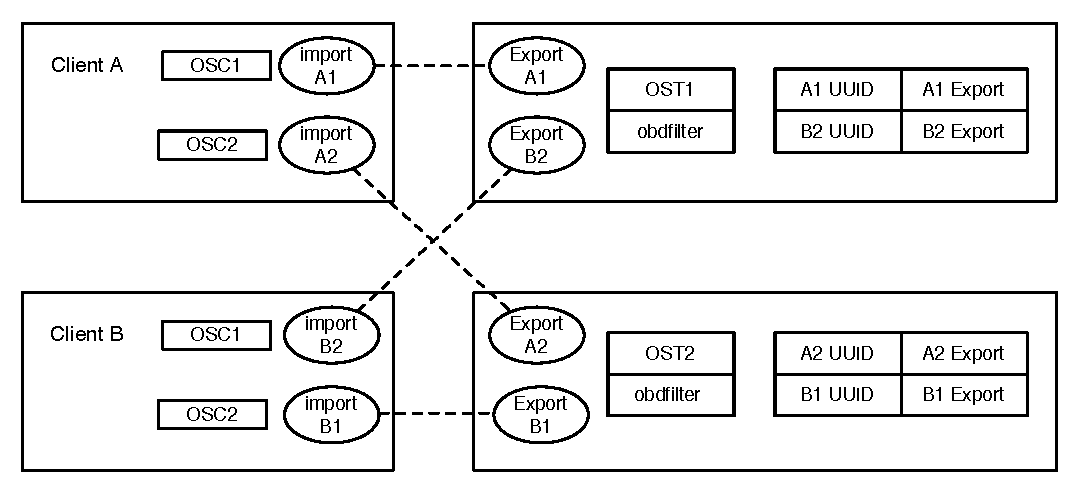
\includegraphics[width=4.5in]{img/obdfilter_conns}
\caption{Import and export connections between an OSC and obdfilter.}
\label{fig:obdfilter_conns}
\end{figure}

The obdfilter provides the following functions:

\begin{itemize}
  
  \item handles create request, presumably from MDS for file data
  objects.

  \item handles read and write requests, from OSC clients.

  \item handles connect and disconnect requests from lower Portal RPC layer for
  established exports and imports.

  \item handles destroy (which involves both client and MDS) requests.

\end{itemize}

\subsubsection{File Deletion}

The destroy protocol is as follows. First, the client decides to remove a file and
this request is sent to MDS. MDS checks the EA striping and uses \url{llog}
to make a transaction log. This log contains the following:
$<$\textit{unlink object 1 from ost1, unlink object 2 from ost2, etc.}$>$.
Then, MDS sends this layout and transaction log back to the client. The
client takes this log and contacts each OST (actually obdfilter) to unlink each
file object. Each successful removal is accompanied by a confirmation or
acknowledgment to the unlink \url{llog} record. Once all unlink llog records on
MDS have been acknowledged, the file removal process is completed.


\subsubsection{File Creation}

As discussed earlier in Section \ref{sec:ost-and-obdfilter}, all requests are
handled by OST and obdfilter together.  Now, we will walk through the handling
of a create request. The first portion of request handling is done inside
\url{ost_create()} as follows.

\begin{enumerate}

\item Prepare the size of reply message. It is composed of two records and thus
requires two buffers. The first record is for portal rpc body, and the second,
for the ost reply body.

\begin{Verbatim}
__u32 size[2] = { sizeof(struct ptlrpc_body), sizeof(*repbody)};
\end{Verbatim}

\item Get a pointer to the request body from the original request and do
byte swapping when necessary.

\begin{Verbatim}
struct ost_body *body = lustre_swab_reqbuf(req, REQ_REC_OFF,
            sizeof(*body), lustre_swab_ost_body);
\end{Verbatim}

The last parameter is the swab handler, which is called only when the swapping is
necessary. Client side uses native byte order for its request, along with a
pre-agreed magic number. Server side reads the magic number to decide if a swap
is needed.

\item Do the actual space allocation, and fill in preliminary header
information.

\begin{Verbatim}
rc = lustre_pack_replay(req, 2, size, NULL);
repbody = lustre_msg_buf(req->rq_repmsg, REPLY_REC_OFF,sizeof(*repbody));
\end{Verbatim}

After the first call, \url{req->rq_repmsg} points to the newly allocated
space. The second call assigns \url{repbody} of the starting address for the buffer
of the reply body.

\item Finally, it fills in the reply body with exactly the same contents as a
request body and passes on to obdfilter for further processing.

\begin{Verbatim}
memcpy(&repbody->oa, &body->oa, sizeof(body->oa));
req-rq_status = obd_create(exp, &repbody->oa, NULL, oti);
\end{Verbatim}

\end{enumerate}

For the create request, the entry point for obdfilter is through
\url{filter_create()}. 

\begin{Verbatim}
static int filter_create(struct obd_export *exp, struct obdo *oa ..)
\end{Verbatim}

We ignore the processing related to \url{struct lov_stripe_md **ea} and
\url{struct obd_trans_info *oti} because the former is a legacy code and
is unlikely to be used in the future.

\begin{enumerate}

\item First, save the current context and assign this client its own operation
context. This is for specifying necessary information for the thread if it
wants to access the backend filesystem. It is like a sandbox limiting the
reach of server threads when processing requests from clients; it stores
``filesystem root'' and ``current working dir'' for the server thread (not
obtained from the client, of course, but rather dependent on which OST
we are working on).


\begin{Verbatim}
obd = exp->exp_obd;
put_ctxt(&saved, &obd->obd_lvfs_ctxt, NULL);
\end{Verbatim}

\item If the request is for recreating an object, then we cancel all extent
locks on the recreated object by acquiring the lock on the object and call on
\url{filter_recreate()} to do the actual job. Otherwise, we follow the normal
flow of precreating objects.  The reason for precreating is that, conceptually,
when MDS asks an OST for creating an object, OST doesn't just create one
object, it creates multiple objects with object id assigned. These batch
created objects have a disk size of zero.  The goal is, when MDS responds to a
client request next time for creating new file, it doesn't have to send a
request to OST again to present the layout information to client. By taking a
look at the pool of precreated objects from each OST, MDS may already have
all the information needed to reply to the client. 

\begin{Verbatim}
if (oa->o_valid & OBD_MD_FLFLAGS) && 
        (oa->o_flags & OBD_FL_RECREATE_OBJS)) {
    rc = ldlm_cli_enqueue_local(obd->obd_namespace, &res_id, ... );
    rc = filter_recreate(obd, oa);
    ldlm_lock_deref(&lockh, LCK_PW);
} else {
    rc = filter_handle_precreate(exp, oa, oa->o_gr, oti);
}
\end{Verbatim}

Here, \url{rc} returned from precreate handler is either a negative, indicative
of an error, or a non-negative number, representing the number of files created.

\item Now, we take a closer look at the function of precreate: 

When a client contacts an OST with a precreated object id, OST knows that this
object id now is activated. However, this presents a problem such that, if the MDS
has failed, it now has stale information on precreated
objects. To resolve this conflict, when MDS is restarted, it checks its records
on unused precreated objects and sends requests to OSTs to delete these
objects (\textit{delete orphans}). The obdfilter takes these requests and
skips those objects that are actually in use (but out of synchronization with
MDS's own record) and removes the rest of it. This is the first part of what
\url{filter_handle_precreate()} will do:

\begin{Verbatim}
if ((oa->o_valid & OBD_MD_FLFLAGS) && 
    (oa->o_flags & OBD_FL_DELORPHAN)) {
    down(&filter->fo_create_lock);
    rc = filter_destroy_precreated(exp,oa,filter);
    ...
} else {
    rc = filter_precreate(obd, oa, group, &diff);
    ...
}
\end{Verbatim}

\item Finally, the create request is passed onto \url{fsfilt} and is completed by
a VFS call. The process will later go through more steps, such as getting hold
of parent inode, transaction setup, etc.

\begin{Verbatim}
rc = ll_vfs_create(dparent->d_inode, dchild, 
                      S_IFREG | S_ISUID | S_ISGID | 0666, NULL);
\end{Verbatim}

\end{enumerate}

%%%% to be added

\begin{comment}

\subsection{Transaction and Error Recovery}

Each client RPC request can potentially open a new transaction on the server
(OST) side. The transaction number is provisioned by the OST to all connecting
clients and mono-increasing until it wraps. Client receives by server reply
RPC, and its \textit{last committed transaction number} field tells the client
if the data associated with the transaction has actually been committed onto
the disk and that determines if client can free up the local memory.

In the event of a server crash and restart, all client will try to re-connect
with the server and then replay requests from the last committed transaction.
If there is any missing client, then its last committed transaction will
become the \textit{bottleneck} as the server can only replay transactions upto
that number. Further, if the recovery timeouts because of the missing clients,
all other clients will be evicted (their states and locks would be discarded).
In 1.6 branch, this collateral damage is quite severe and in some cases not
necessary. In Lustre 1.8, it has been addressed by VBR, but that is another
story.


\end{comment}



%\section{Lustre Lite}

In this section, we describe how Lustre Lite connects and fits into
Linux VFS, which is necessary for  supporting VFS semantics and the POSIX
interface. To summarize, Lustre Lite provides the following functions through
a method table:

\begin{itemize}

  \item Lustre specific file operations, through
  \url{ll_file_operations}.

  \item Lustre specific dentry operations, through \url{ll_d_ops} and
  its cache.

  \item Lustre specific directory operations, through
  \url{ll_dir_operations}.

  \item Lustre specific inode operations, through
  \url{ll_dir_inode_operations} and \url{ll_file_inode_operations}.

  \item Lustre specific file mapping operations, through
  \url{ll_file_vm_ops}.

  \item And many others, such as Lustre super block operations, address
  spaces, etc.

\end{itemize}

\begin{figure}[hbt]
\centering
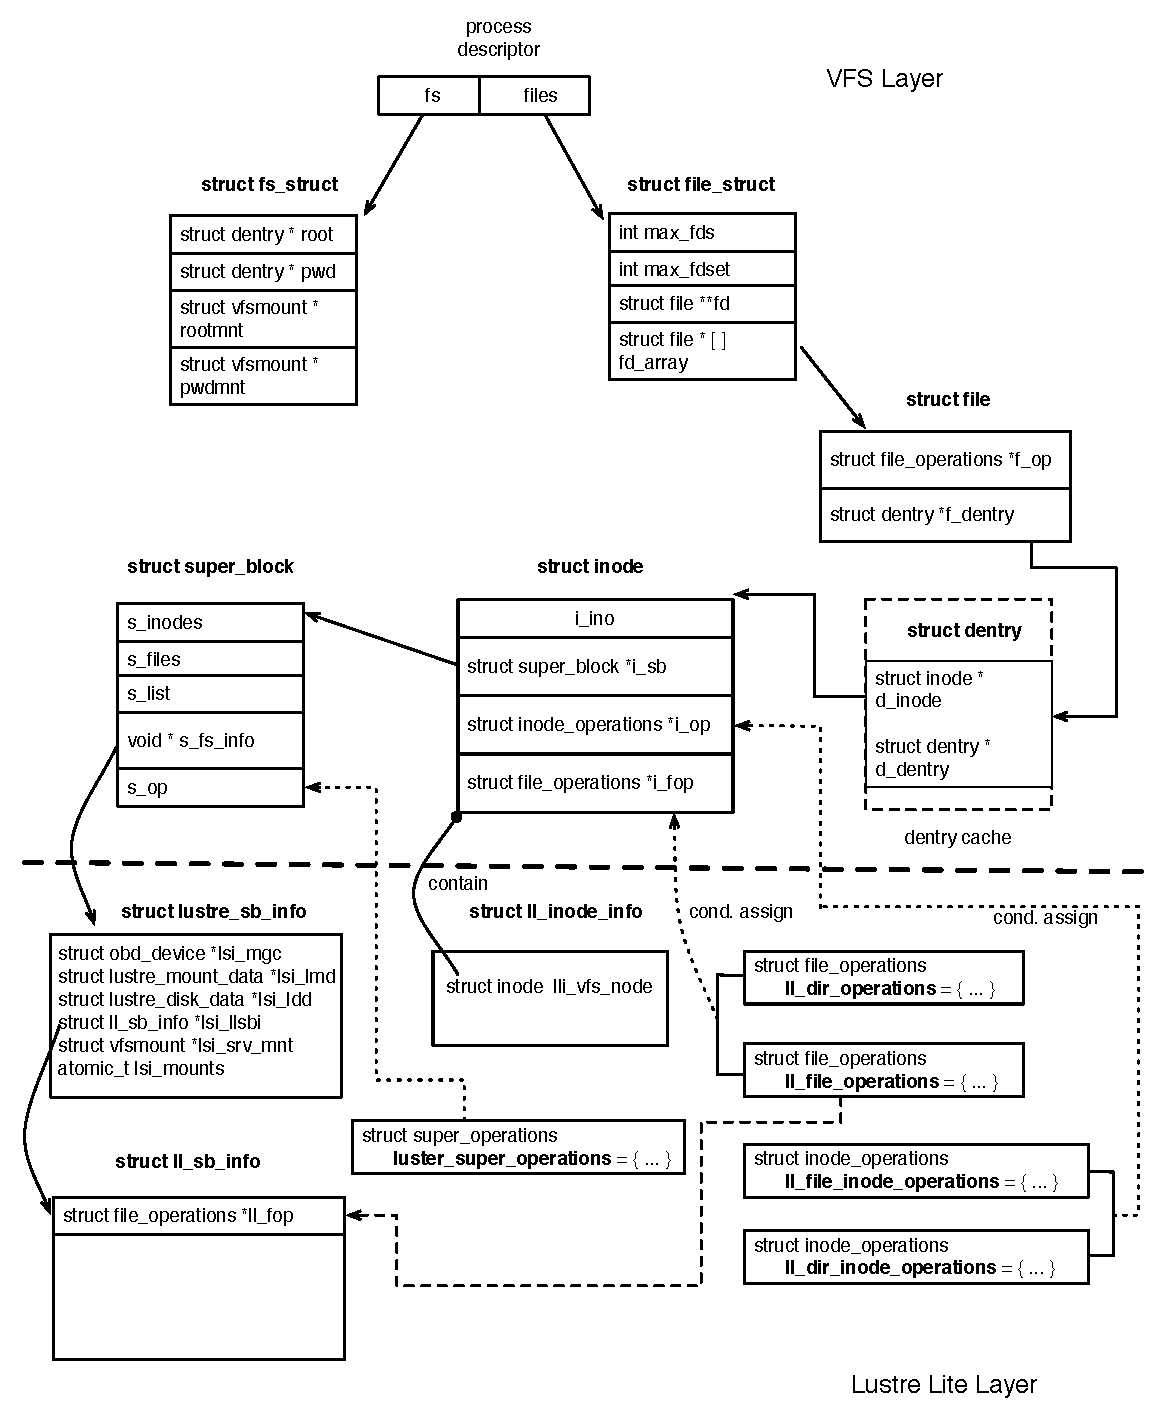
\includegraphics[width=5in]{img/lustre_vfs}
\caption{Hooking up Lustre with Linux VFS.}
\label{fig:vfs}
\end{figure}

\subsection{VFS Connection}
\label{sec:vfsreg}

Figure \ref{fig:vfs} presents an overall picture of how various data structures
are connected. Some highlights are explained below.

A process maintains a list of associated open files. Each open file has an
in-memory representation known as the \url{file} object. It stores the
information necessary to interact between an open file and process.  To the
userland, this is presented by a file handle, \url{fd}. This data structure
contains a field, \url{f_op}, that acts like a switchboard or pointer to a
method table that provides functions specific to each filesystem. So a file
read using system call \url{sys_read()} becomes: 

\begin{Verbatim} 
file->f_op->read(...);
\end{Verbatim}

\subsubsection{Dentry Object}

Another important field defined in the \url{file} structure is \url{f_dentry},
which points to a dentry object (\url{struct dentry}) stored in a dentry
cache, also known as the \textit{dcache}. Essentially, VFS will create a
dentry object  the first time a file or directory is about to be accessed. If
this is a non-existent file/directory, then a negative dentry will be
created.  As an example, take the following pathname:
\url{/home/bob/research08}; it is composed of four path components:
\url{/}, \url{home}, \url{bob}, and \url{research08}.  Correspondingly, the
path lookup will create four \url{dentry} objects for each component.  Each
dentry object associates \textit{the} respective component with its inode
through field \url{d_inode}.

The inode object stores information about a specific file, uniquely identified
by an inode number. ULK3\footnote{Understanding the Linux Kernel, the third edition.}
has exhaustive listings of field definitions for inode structure. What is
important to know is that  (1) \url{i_sb} points to the VFS superblock; (2)
\url{i_op} is the switchboard for inode operations such as: 

\begin{Verbatim}
    create(dir, dentry, mode, nameidata) 
    mkdir(dir, dentry, mode) 
    lookup(dir,dentry,nameidata)
    ...
\end{Verbatim}

The first method creates a new disk inode for a regular file, associated
with a dentry object in some directory. The second method creates a new
inode for a directory associated with some dentry object in some
directory. And the third one searches a directory for an inode
corresponding to a filename included in a dentry object.

\subsubsection{Lustre Superblock}

VFS layer defines a generic superblock object (\url{struct super_block}),
which stores information about the mounted filesystem. One particular field
\url{s_fs_info} points to superblock information that belongs to a specific
filesystem. In the case of Lustre, this filesystem specific data is
represented by the structure \url{lustre_sb_info}, which stores information
needed for mounting and unmounting Lustre filesystem. It further connects to
another structure \url{ll_sb_info}, which contains more Lustre
Lite\footnote{We use Lustre Lite and llite interchangeably.} specific
information about filesystem state only for clients.

Lustre specific superblock operation is defined in struct variable
\url{lustre_super_operations}. \footnote{See more details in
\url{lustre/llite/super25.c}, which is actually for kernel 2.6} The initialization of
\textit{correct} superblock operations takes place when we initially
establish the in-memory superblock data structure in function
\url{client_common_fill_super()}:

\begin{Verbatim}
    sb->s_op = &lustre_super_operations;
\end{Verbatim}

It is worth mentioning that when creating Lustre files, the
\url{alloc_inode()} superblock method is implemented by \url{ll_alloc_inode()}
function. It will create a Lustre specific inode object \url{ll_inode_info} and
return the VFS inode embedded in it. Pay attention to the particular way in
which the generic VFS inode and Lustre inode interconnect with each other:
this method creates and fills the VFS inode structure along with extra state
information the Lustre filesystem needs, but it only returns the VFS inode
structure \url{&lli->lli_vfs_inode} embedded in \url{lli}. \footnote{The fact
that we allocate one big structure that holds both VFS inode and Lustre
private state information is an implementation detail, and it is not necessary
to be this way.  It used to be that private state info was allocated
separately and a pointer from VFS inode was used to access it.}

\begin{Verbatim}
    static struct inode **ll_alloc_inode(struct super_block *sb)
    {
        struct ll_inode_info *lli;
        ...
        return &lli->lli_vfs_inode;
    }
\end{Verbatim}


To retrieve the parent structure from a child structure, Lustre defines a
helper method \url{ll_i2info()}, which essentially invokes kernel macro
\url{container_of} by:

\begin{Verbatim}
    /* parameters of macro: ptr, type, memeber */
    return container_of(inode, struct ll_inode_info, lli_vfs_inode);
\end{Verbatim}

\subsubsection{Lustre inode}

The initialization of correct inode and file/dir functions takes
place when inode is being filled in during \url{ll_read_inode2()}.  There are
four struct variables defined for it, and two of these are for inode
operations: \url{ll_file_inode_operations} and \url{ll_dir_inode_operations}.
Two of these are for file/directory operations, \url{ll_file_operations}, and
\url{ll_dir_operations}. In each case, file and directory each has its own
set, and which to assign depends on the inode or the file itself.
\footnote{These variables are scattered in various places such as
\url{file.c}, \url{dir.c}, \url{namei.c}.} The following snippet shows an 
example of a definition for file operations:

\begin{Verbatim}
/* in dir.c */
struct file_operations ll_dir_operations = {
        .open     = ll_file_open,
        .release  = ll_file_release,
        .read     = generic_read_dir,
        .readdir  = ll_readdir,
        .ioctl    = ll_dir_ioctl, ...
};
/* in file.c */
struct file_operations ll_file_operations = {
	.read	= ll_file_read,
	.write	= ll_file_write,
	.open	= ll_file_open, ... 
\end{Verbatim}

For example, if the inode to be created is a file, then \url{i_fop} will be
assigned as \url{ll_file_operations}; if the inode to be created is a
directory, then \url{i_fop} will be assigned as \url{ll_dir_operations}:

\begin{Verbatim}
if (S_ISREG(inode->i_mode)) {
    inode->i_op = &ll_file_inode_operations;
    inode->i_fop = sbi->ll_fop;
    ...
} else if (S_ISDIR(inode->i_mode)) {
    inode->i_op = &ll_dir_inode_operations;
    inode->i_fop = &ll_dir_operations;
    ...
\end{Verbatim}

A general observation on the pattern: the pointer for the method table is
initialized and established properly by the party or the function that
is creating the new instance of it.

\subsection{Path Lookup}

Path lookup is a relatively complex task and one of the most important and
frequently performed. Linux VFS does most of the heavy lifting; we want to
emphasize the junction at which Lustre does specific things.  In this
section, we outline basic steps with enough details to follow the main
thread of the code but skip many branches one has to take care of in real
code, such as:

\begin{itemize}
\item the path name contains component of \url{.} and \url{..},
\item the path name contains symbolic links, which may induce circular
reference,
\item the access rights and permission check,
\item the path name contains mount point of another filesystem,
\item the path name contains not-yet-existing file,
\item \url{LOOKUP_PARENT} flag set,
\item the path name does not have a trailing slash.
\end{itemize}

Lookup can be invoked from \url{sys_open()} call, the usual call path from
there is to do \url{filp_open()} and \url{open_namei()}. It is this last
function that initiates \url{path_lookup()} call. In particular, if a file is
opened with \url{O_CREAT} flag in the parameter for access mode, the lookup
operation will be set with \url{LOOKUP_PARENT}, \url{LOOKUP_OPEN}, and
\url{LOOKUP_CREATE}. The end result of path lookup is either: \begin{itemize}
\item return dentry object of last path component if it exists; or \item
return dentry object of next-to-last path component if it does not, as in the
case of creating a new file. From there, you can allocate a new disk inode by
invoking the \url{create} method of the parent inode.  \end{itemize}

Now we focus on the lookup specifics. If the path starts with \url{/}, then it
is an absolute path: search starts with the process root directory in
\url{current->fs->root}. Otherwise, a search starts with \url{current->fs->pwd}.
We also know the dentry object as well as its inode of beginning directory at
this point (refer back to figure \ref{fig:vfs} to see why). The
\url{nameidata} keeps track of the last resolved path component with \url{dentry}
and \url{mnt} fields.  Initially, they are assigned with \textit{starting
directory}. The core lookup operation is performed by \url{link_path_walk(name,
nd)}, where \url{name} is the path name, \url{nd} is the address of the 
\url{nameidata} structure.

\begin{enumerate}

\item Consider next component to be resolved; from its name, compute
32-bit hash value to be used when looking in the dentry cache hash
table.

\item Set \url{LOOKUP_CONTINUE} flags in \url{nd->flags} to denote that
there are more components to be analyzed.

\item Invoke \url{do_lookup()} to search dentry object for the path
component. If found (skip revalidation), then this path component
has been resolved, and move on. If not found, then invoke \url{real_lookup()}. At the
end of the cycle, the \url{dentry} and \url{mnt} field of local dentry
variable \url{next} will point to, respectively, the dentry object and
the mounted filesystem object of the path component we attempt to resolve.

\item If the above \url{do_lookup()} reaches the last component of
the pathname, and assuming that it is not a symbolic link as assumed
at the beginning, then this is our destination. All we need to do is to store
the dentry object and mnt info in the passed nameidata \url{nd} and return
without error:
\begin{Verbatim}
    nd->dentry = next->dentry;
    nd->mnt  = next->mnt;
\end{Verbatim}

\end{enumerate}

Lustre specific operation is handled in the \url{real_lookup()} call.  A
dentry is created by VFS and is passed into the filesystem specific lookup
function.  Lustre's lookup responsibility is to locate or create a
corresponding inode and fill it with correct information. If inode could not
be found, then the dentry still remains, only it has a \url{NULL} inode pointer.
Such dentries are called \textit{negative} meaning there is no such file with
this name. The particular code segment for this switching is given below.

\begin{Verbatim}
    struct dentry *result;
    struct inode *dir = parent->d_inode;
    ...
    result = d_lookup(parent, name);
    if (!result) {
        struct dentry *dentry = d_alloc(parent, name, nd);
        if (dentry) {
            result = dir->i_op->lookup(dir,dentry,nd);
            ...
     }
\end{Verbatim}

Now the lookup is passed on Lustre's side, and follow-on operations might
involve contacting MDS for more information.

There is also a \url{cached_lookup} path that calls in a \url{->revalidate}
method provided by the Lustre. This method verifies that the cached dentry/inode is
still valid and does not need to be updated from the server.

\subsection{I/O Path}

This section starts with discussions on three I/O paths traveled by Lustre:
Async I/O, Group I/O, and Direct I/O. Then we discuss how Lustre interfaces
with VFS by surrendering control of I/O (in most cases) to VFS,
which does more preparations and then reads/writes data on a page-by-page
basis through address space methods, which are in turn provided by Lustre. So
think of this as a process of: VFS to llite through hooks, llite then calls
into VFS for processing help, and VFS then hands control back to llite --
an in and out intertwined process. 

\subsubsection{Asynchronous I/O}

This is probably the most traveled I/O path in Lustre, and we will provide a
top-down description on the write process. Read operation is very similar. The
registered file write operations for VFS are discussed in Sec.
\ref{sec:vfsreg}.

\begin{enumerate}

\item The \url{writev()} is for older kernels, newer ones will use \url{aio_write()}.
Our entry point of analysis is \url{ll_file_write()}. This function defines a
\url{iovec} with base pointing to the buffer provided at the user space, and length
is the number of bytes to write. 
\begin{Verbatim}
struct iovec local_iov = { .iov_base = (void __user *) buf, 
                           .iov_len  = count };
\end{Verbatim}

Another structure initialized here is \url{kiocb}, which records the status of
the I/O. Passing in as parameters both \url{iovec} and \url{kiocb}, it invokes
either \url{ll_file_writev()} or \url{ll_file_aio_write()} depending on the
kernel version. In our case, we follow the latter. Codewise, both functions
are implemented as one, only with slightly different prototype declarations:

\begin{Verbatim}
#ifdef HAVE_FILE_WRITEV
static sszie_t ll_file_writev( 
                            struct file *file, 
                            const struct iovect *iov,
                            unsigned long nr_segs, 
                            loff_t *ppos) {
#else /*AIO stuff */
static ssize_t ll_file_aio_write(  
                            struct kiocb *iocb,
                            const struct iovec *iov,
                            unsigned long nr_segs,
                            loff_t pos)
{
    struct file *file = iocb->ki_filp;
    loff_t *ppos = &iocb->ki_pos;
#endif 
\end{Verbatim}


\item The key to understanding this function (\url{ll_file_aio_write()}) is
that Lustre breaks the write into multiple chunks based on the stripe size,
then asks for a lock on each chunk in a loop. \footnote{The lock granularity
is page unit, which is useful when you do small I/O. Normally, you would
request a lock on stripe size. One exception is if it is \url{O_APPEND} write,
then the lock is for the entire file.} This is to avoid complications when you
have to ask a lock on a large extents. Although we said earlier that LOV is
the layer that handles stripe info, Lustre Lite is very much aware of that as
shown in this case -- you can see how closely coupled they are. The stripe
info is obtained by: 

\begin{Verbatim} 
struct lov_stripe_md *lsm = ll_l2inof(inode)->lli_smd; 
\end{Verbatim}

Lustre controls the size of each write by setting up a copy of the original iov
control structure, \url{iov_copy}, then goes back and asks one of common
routines in the kernel to drive the write:

\begin{Verbatim}
retval = generic_file_aio_write(iocb, iov_copy, nrsegs_copy, *pppos);
\end{Verbatim}

We tally the number of bytes to write in \url{*iov} and use \url{count} to
track the number of bytes remaining to be written. This is repeated until an
error is hit or all bytes are written.

Before we make a generic write routine, in addition to getting a lock by
calling \url{ll_file_get_tree_lock_lov()},  there are a few corner cases this
function needs to deal with:

  \begin{itemize}

  \item If user-application opens the file with \url{O_LOV_DELAY_CREATE}, but
  starts to write without first calling \url{ioctl} to set it up, then we need
  to fail this call.

  \item If user-application opens the file with \url{O_APPEND}, then we need to
  get a lock on the entire content: \url{lock_end} is set with
  \url{OBD_OBJECT_EOF}, or -1 to represent the end of the file.

  \end{itemize}

\item \url{generic_file_aio_write()} is just a wrapper for
\url{__generic_file_aio_write_nolock()}; both functions have been described in
ULK3, and we will not dwell on it here. Since direct I/O is not covered in
this section, the write flow goes into \url{generic_file_buffered_write()}.
This is where the write is further broken into pages, and page cache
is allocated. The main body of work is performed in the loop given below.

\begin{Verbatim}
do {
    ...
    status = a_ops->prepare_write(file, page, offset, offset+bytes);
    ...
    copied = filemap_copy_from_user(page, offset, buf, bytes);
    ...
    status = a_ops->commit_write(file, page, offset, offset+bytes);
    ...
} while (count);
\end{Verbatim}

First, we prepare the page write through the Lustre registered method. The
preparation involves checking if the starting position is aligned at the
beginning and if it needs to be read from disk first (of course, there is no
local disk operation here in Lustre, but VFS sees it that way). Then it copies
a page worth of data from user space to the kernel. Finally, we once again ask
Lustre specific method to write the page out. So the control is passed in and
out of Lustre code twice.

There are a few interesting points to make on page and boundary management. Let's
say the logical file position for write is 8193 and the page size is 4KB. As
this is a page-based write (both prepare write and commit write are
page-based), it first calculates page index (2) and page offset (1), and
\url{bytes} are the maximum bytes you can write in that page.  However, if the
remaining \url{count} is less than that, we need to adjust it by the exact
number of bytes we will write for this page.

\begin{Verbatim}
index = pos >> PAGE_CACHE_SHIFT;
offset = (pos & (PAGE_CACHE_SIZE -1));
bytes = PAGE_CACHE_SIZE - offset;
bytes = min(bytes, count);
\end{Verbatim}

This calculated logical page index will be used to locate or allocate a page in
the page cache and be associated with this file mapping:

\begin{Verbatim}
struct address_space *mapping = file->f_mapping;
page = __grab_cache_page(mapping, index, &cached_page, &lru_pvec);
\end{Verbatim}

A small digression: The \url{__grab_cache_page()} is a helper function that
is only used for generic file write requests.  The basic flow of this function
is to first check if such a page already exists in the pagecache and return it
if so.  Otherwise, it allocates a new page by invoking
\url{page_cache_alloc()} and adds it to page cache
(\url{add_to_page_cache()}). However, another thread might
allocate a page at this offset just between the last check and now, so adding
to pagecache can fail. In that case, we need to check and retrieve the page
from pagecache again:

\begin{Verbatim}
repeat:
    page = find_lock_page(mapping, index);
    if (!page) {
        ... page_cache_alloc(mapping);
        err = add_to_page_cache(*cached page, mapping, index, GFP_KERNEL);
        if (err == -EEXIST)
            goto repeat;
\end{Verbatim}

A small optimization is made here at the cost of polluting the code: if a
just-allocated page cannot be added to the page cache as shown, instead of
returning it, it keeps it in \url{cached_page}, so next time when a new page is
requested, we don't have to call the allocation function again.



\item Now we can move to prepare write. It is declared as given below.

\begin{Verbatim}
int ll_prepare_write(struct file *file, struct page *page, 
		     unsigned from, unsigned to)
\end{Verbatim}

The~\url{ll_prepare_write()}is invoked with~\url{from} set as the~\url{offset}
and~\url{to} set as the~\url{offset + bytes}. This is exactly the boundary
issue we discussed above.  Overall, this method is to
ensure that \textit{the page is up to date}, and if this is not a full page write,
then read in the partial page first. 

A few structs are used in this function; their meanings are as follows:

\begin{description}

\item[\url{struct obdo}] is for \textit{on the wire} representation of a Lustre
object and its related information.

\item[\url{strut brw_page}] is for describing the state of the page for
sending.

\item[\url{struct obd_info}] is for passing parameters between Lustre layers.

\end{description}

Also in this method, we need to check the end of file (EOF) for cases like
\textbf{partial page write}: if EOF falls within the page (write beyond EOF),
then we need to fill in non-overwriting portions with zeros; otherwise, we need
to preread it.

\item Next, the LOV initiates preparing page by \url{lov_prep_async_page()}.

There are three structs defined at each layer a page write needs to go through.
At the Lustre Lite layer, there is the \url{ll_async_page} (LLAP).  The LOV
defines the \url{lov_async_page} (LAP) and the \url{osc_async_page} (OAP).

\item If the write operation is async, it will be handled by
\url{osc_queue_async_io()}, and internally it calls function
\url{osc_enter_cache()}, which does page accounting to ensure we do not have
more dirty pages than allowed, and blocks on attempts to add extra dirty pages.
It also enforces grants in similar manner.

Therefore, in (at least) two conditions an OAP will not be able
to go into the cache:

  \begin{itemize}

  \item If the size of the cache is less than 32MB, then it is O.K. to put
	OAP into cache, return 0; otherwise, return an error code.

  \item If the grant is not sufficient on the client side, then again return an
	error code. Upon each OSC client's initialization, one can assume that the OST
	server side granted the client some space. A \textbf{grant} is just a number
	promised by the server that this client can flush out this much data and
	knowing the server can deal with it.  The initial grant is 2MB, which is two
	RPC's worth of data. Then, write request is issued by the client, and it can ask
	for more grant if needed. At the same time, along with each data transfer or
	write, client needs to keep track of this grant and not to overrun it.

  \end{itemize}

If the page is unable to get into the buffers, a group I/O or synchronous I/O
will be tried later.    

\item After the OAP caching check is done, \url{loi_list_maint()} is called to put
it on the proper list, and readying it for either read or write actions.

\item Function \url{osc_check_rpcs()} builds RPCs for each object in
\url{lov_oinfo}. Note that each RPC can carry content for only one data
object. 

\end{enumerate}

\subsubsection{Group I/O (or Synchronous I/O)}

Group I/O is triggered when an OAP page cannot be successfully
put into cache, most likely because of an insufficient grant. In that case,
Lustre Lite will create a structure \url{obd_to_group} to hold OAP. This page
will then be added to the client obd's ready list, with the URGENT flag set.
Finally, \url{oig_wait()} would be invoked and wait for group I/O to finish. 

Notice that group I/O waits on the operation; therefore, it is also known
as~\textbf{synchronous} I/O. Second, all group I/O is urgent I/O as well as
read operations.  In contrast, in~\textbf{asynchronous} I/O, the OAP cache
(when admitted) will go into the write list.

It is also worth noting that except direct and lockless I/O, all reads are done
as group I/O. Direct I/O is briefly discussed below. Lockless I/O is a special
kind of I/O (now disabled except in liblustre) where clients do not get any
locks but instead instructs the server to take the locks on the client's
behalf.

\subsubsection{Direct I/O}

For direct I/O, VFS passes an \url{iovec}, which describes a segment of data to
transfer. It is simply defined by a start address \url{void * iobase} and a
size, \url{iov_len}. Direct I/O requires that the start address
be page-aligned.

Lustre Lite operates on each page and invokes \url{ll_direct_IO_26()} and
\url{obd_brw_async()}, and this essentially gets converted to
\url{osc_brw_async()} calls that later will be used for building RPC requests.


\subsubsection{Interface with VFS}

At the top level of VFS in general and Lustre Lite in particular, there are
several places where you can register your own read and write methods, all
through address space operation struct. For read operations, it is
\url{readpage()} and its the vector version of \url{readpages()}. For write, it
is a bit more complicated.  The first entry point is \url{writepage()}, which
can be triggered by:

\begin{itemize}

  \item When memory pressure crosses the threshold, VM will trigger 
  the flushing of dirty pages.
  
  \item When a user application does an \url{fsync()} and forces the flushing of
  dirty pages.

  \item When a kernel thread does the periodical flushing of dirty pages. 

  \item When the lock on the page is revoked (block request) by the Lustre
  lock manager, the dirty page therefore must be flushed.

\end{itemize}

The implementation of \url{readpage()} and \url{writepage()} are optional, and
not all filesystems support them. However, these methods are needed to take
advantage of default read/write actors in kernel (\textit{i.e.}, the generic
implementation of \url{do_generic_file_read()} and
\url{do_generic_file_write()}). It simplifies the interactions with kernel
cache and VM. Also, both methods are needed to provide~\url{mmap} support.  

Filesystem registers the functions \url{prepare_write()} and \url{commit_write()}
via an address space object as well.\footnote{Linux Kernel 2.6 introduces
\url{write_begin()} and \url{write_end()}} So, an address space object can be
characterized as the bridge from file space to storage space.

The address space operation in Lustre is defined in \url{lustre/llite/rw26.c}:

\begin{Verbatim}
struct address_space_operations ll_aops = {
    .readpage           =   ll_readpage,
    .direct_IO          =   ll_direct_IO_26,
    .writepage          =   ll_writepage_26,
    .set_page_dirty     =   __set_page_dirty_nobuffers,
    .sync_page          =   NULL,
    .prepare_write      =   ll_prepare_write,
    .commit_write       =   ll_commit_write,
    .invalidatepage     =   ll_invalidatepage,
    .releasepage        =   ll_releasepage,
    .bmap               =   NULL
};
\end{Verbatim}

There is an \url{*f_mapping} field in \url{file} object pointing to the address
space object associated with the file. The connection is established at file
object creation. 

\begin{figure}[htb]
\centering
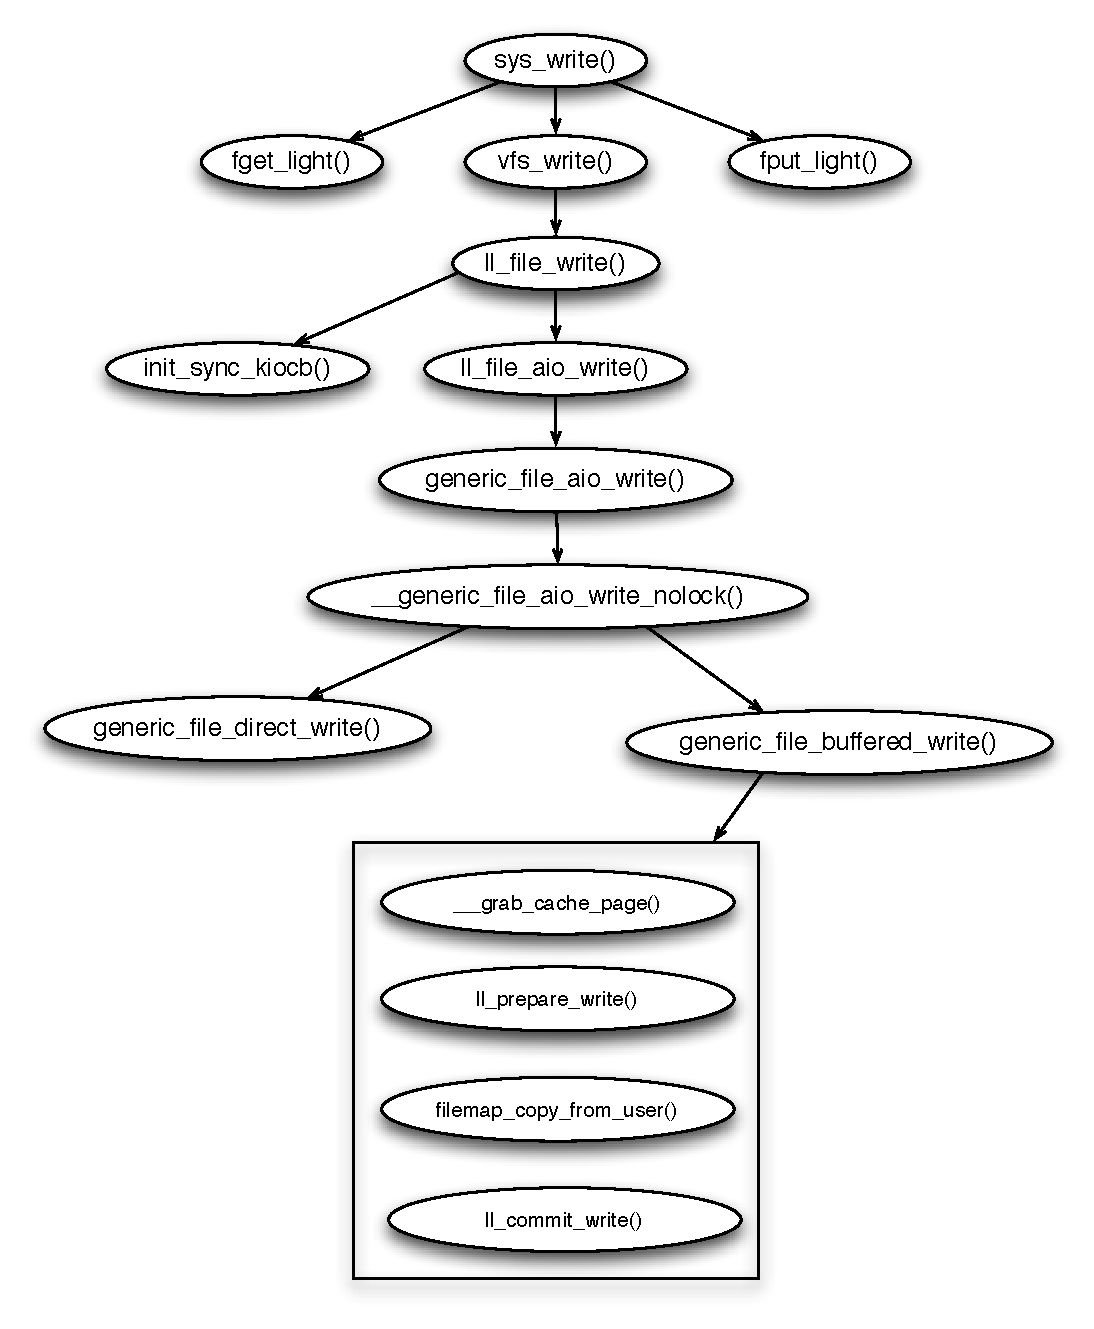
\includegraphics[width=4.5in]{img/lite_write}
\caption{System call graph on the write path as in Linux kernel 2.6.22-14.}
\end{figure}


\subsection{Read-Ahead}

Lustre client read-ahead happens in read-page and is controlled by a
structure, \url{ll_readahead_state}, which is defined in
\url{lustre/llite/llite_internal.h}. This is a per-file structure and encodes
the following information:

\begin{itemize} 

\item \textbf{Read history} (a) how many contiguous reads have happened; (b)
if it is stride read mode, then how many contiguous stride reads have happened;
and (c) stride gap and stride length.

\item \textbf{Read-ahead} windows (i.e., read-ahead window starting and end
points). The more contiguous read happens, the longer the read-ahead window
grows.

\item State information that helps to \textbf{detect read-ahead pattern}.

\end{itemize}

The read-ahead algorithm is described below where each client could read-ahead
a maximum of 40MB:

\begin{enumerate}

\item In read-page (\url{ll_readpage}), the read-ahead state of the file will be
updated according to the current status.
    \begin{enumerate}
     
    \item If this page offset is located in a contiguous window (in +8, -8 window
	with the last page), then \url{ras_consecutive_requests} (defined by
	\url{ll_readahead_state}) will increase by 1. If it is the first page of this
	read, the read-ahead window length will increase by 1MB.  So if the read is
	contiguous, the read-ahead window increases with an increasing number of read
	opeartions.


    \item If this page is not inside the contiguous window, then it will check
    whether it is in stride-read mode. In this case, it will compare current
    stride length/stride gap with past history. If they are equal, then
    \url{ras_consecutive_stride_requests} will be increased by 1. If it is the
    first page of this read, stride read-ahead window will also increase by
    1MB.

    \item If page is neither in contiguous window nor in stride-contiguous
    window, then all the read-ahead state will be reset. For example,
    \url{ras_consecutive_pages} and \url{ras_consecutive_requests} will be
    reset to 0.

    \end{enumerate}

\item Next, read page will do real read-ahead according to the state updated
in the previous step.

     \begin{enumerate}

      \item Increase the read-ahead window and try to cover all the pages for
      this read. This explains why large reads perform better than small
      reads.
       
       \item Adjust the read-ahead window according to the real file length and
       calculate how many pages will be read in this read-ahead.
       
      \item Do actual read-ahead.
    \end{enumerate}

\end{enumerate}

There is a read-ahead stats file in the proc
(\url{/proc/fs/lustre/llite/XXXXX/read_ahead_stats}) where states of read
ahead can be viewed.



%\section{LNET: Lustre Networking}
\label{sec:lnet}

LNET is a message passing API, originated from Sandia Portals.  Although there
are commonalities between the two, they are not the same thing. We will cover the
Lustre LNET without delving into the differences between the two. 

\subsection{Core Concepts}

First, we need to clarify some terminology used throughout the rest of the
section, in particular, the process id, matching entry, matching bits, and
memory descriptor.

\begin{figure}[htb]
\centering
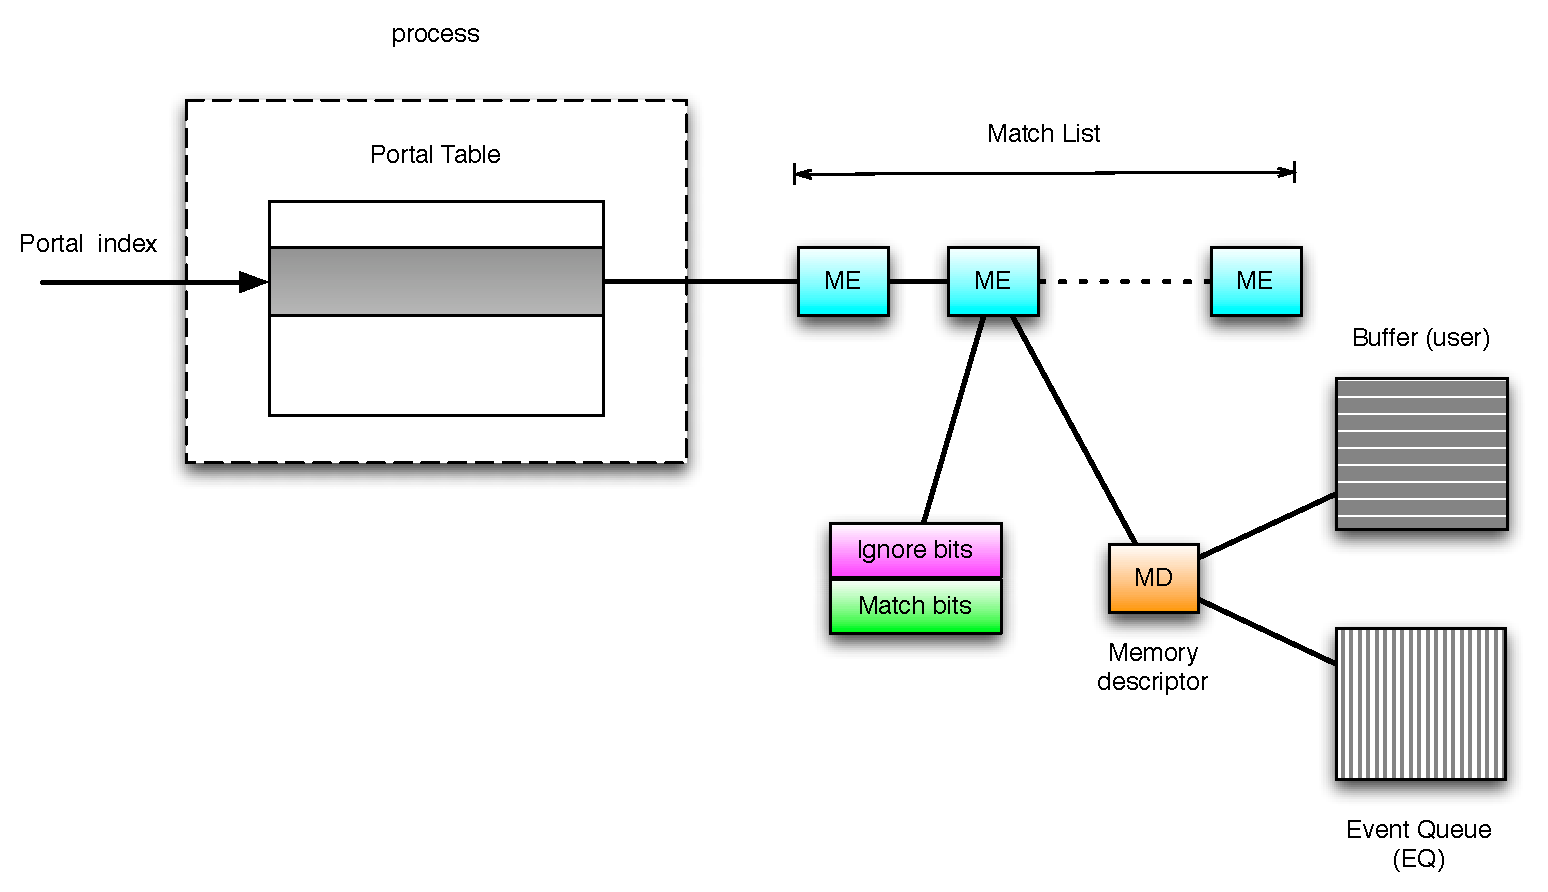
\includegraphics[width=5in]{img/lustre_portal_address}
\label{fig:lustre_portal_address}
\caption{Illustration of Lustre LNET addressing scheme.}
\end{figure}

\subsubsection*{LNET Process Id}

LNET identifies its peers using the LNET process id, defined as follows:

\begin{Verbatim}
typedef struct {
    lnet_nid_t  nid;
    lnet_pid    pid;
} lnet_process_id_t;
\end{Verbatim}

The \url{nid} identifies the id of the node, and \url{pid} identifies
the process on the node. For example, in the case of socket LND (and
for all currently existing LNET LNDs), there is only one instance of LNET
running in the kernel space; the process id therefore uses a reserved ID
(12345) to identify itself.

\subsubsection*{ME: Matching Entry}

A \textit{portal} is composed of a list of match entries (ME). Each ME can be
associated with a buffer, which is described by a memory descriptor (MD). ME
itself defines match bits and ignore bits, which are 64-bit identifiers that
are used to decide if the incoming message can use the associated buffer space.
Figure \ref{fig:lustre_portal_address} illustrates the Lustre LNET addressing
scheme.


\begin{Verbatim}
typedef struct lnet_me {
        struct list_head   me_list;
        lnet_libhandle_t   me_lh;
        lnet_process_id_t  me_match_id;
        unsigned int       me_portal;
        __u64              me_match_bits;
        __u64              me_ignore_bits;
        lnet_unlink_t      me_unlink;
        struct lnet_libmd *me_md;
} lnet_me_t;
\end{Verbatim}

All MEs associated with the portal are linked by the \url{me_list}.  The
\url{me_match_id} defines which remote LNET peer(s) are allowed to access this
ME, and it can be a wildcard that allows open access.

\subsubsection*{MD: Memory Descriptor}

Following the creation of an MD by the upper layer, the LNET layer uses
the~\url{struct lnet_md_t} to reference the MD. The LNET internal
representation is described by \url{struct lnet_libmd_t}.  Per our
understanding, the purpose is to make \url{lnet_libmd_t} opaque to the client
so that they cannot interfere with LNET internal states. They share some of the
common fields, but LNET maintains more states for internal housekeeping.

\begin{Verbatim}
typedef struct {
        void             *start;
        unsigned int     length;
        int              threshold;
        int              max_size;
        unsigned int     options;
        void             *user_ptr;
        lnet_handle_eq_t eq_handle;
} lnet_md_t;
\end{Verbatim}

If a memory buffer described by MD is contiguous, then the address of
\url{start} points to the begining of the memory. Otherwise, it points to the
start of some I/O vectors.  There can be two kinds of I/O vectors: if the
memory is already mapped to virtual memory, it is described by \url{struct
iovec}; otherwise, it is described by \url{lnet_kiov_t}, which may or may not be
mapped to virtual memory, and by definition, it is just a memory page.  MD
options (\url{options}) identifies the type of I/O vectors. It is either
\url{LNET_MD_IOVEC} or \url{LNET_MD_KIOV}. Also, if the MD is describing a
non-contiguous memory, \url{length} then describes the number of entries in the
array.

As mentioned above, \url{struct lnet_libmd_t} is used by LNET internal to
describe the MD along with some other bookkeeping fields:

\begin{Verbatim}
typedef struct lnet_libmd {
    struct list_head    md_list;
    lnet_libhandle_t    md_lh;
    lnet_me_t           *md_me;
    unsigned int        md_length;
    unsigned int        md_offset;
    unsigned int        md_niov;
    union {
        struct iovec    iov[LNET_MAX_IOV];
        lnet_kiov_t     kiov[LNET_MAX_IOV];
    } md_iov;
    ...
}
\end{Verbatim}

It should be obvious that \url{md_me} is the address of the ME entry this MD is
associated with, and it can be \url{NULL}. The \url{md_length} is the total
number of bytes of all segments this MD describes, and \url{md_offset} is the
number of bytes to skip. For a noncontiguous memory, think of it as all being
combined into a virtual contiguous array and you have a logical offset into it.
The \url{md_niov} is the number of valid entries of the I/O vectors described
by either \url{iov} or \url{kiov} in the union struct. \url{md_list} is a
hashtable with handle (\url{md_lh}) as key to locate an MD.

\subsubsection*{Example Use of Offset}

Upon initialization, the server will \textit{post} request buffers (for the request
portal); the buffer is to accommodate incoming client requests. We further
assume that the request buffer is 4KB in size and each request should be 1KB at
most. When the first message comes, the offset is increased to 1KB, and with the
second message, the offset is set to 2KB and so on. So essentially, the offset
is used to keep track of the write position to fend off an overwrite, and this is
the default case. Another case where offset is being used differently will be
described after we talk about MD options.

\subsubsection*{MD Options}

If the MD has the \url{LNET_MD_MANAGE_REMOTE} flag set, then the client can
indicate the offset into the MD for the GET or PUT operations. In the follow-on
API discussion, we describe the offset parameter in the GET and PUT API.
We describe two use cases here: 

\begin{itemize}

\item The router posts a buffer containing the nids for interested clients to read,
with \url{LNET_MD_MANAGE_REMOTE} and \url{LNET_MD_OP_GET} flags set. All clients
will get the buffer with offset as zero since they will get a complete list of nids
on the router.

\item For the case of an early server reply when adaptive timeout is in use,
the client posts one reply buffer before sending out the request. The server first
responds with an early reply with the offset set to zero. This means ``I got your
request, now wait patiently." Later, the server sends the actual reply to the
same buffer with the proper offset.  

\end{itemize}

Another type of attribute associated with the MD defines the operations
allowed on the MD. For example, if the MD only has a get flag
\url{LNET_MD_OP_GET}, then writing into this MD is not allowed. This is
equivalent to the read-only case. And \url{LNET_MD_OP_PUT} means the MD only
allows for a PUT operation, but without the GET flags, it becomes a write-only. 

There are two flags dealing with the case where an incoming message is bigger
than the current MD buffer. The \url{LNET_MD_TRUNCATE} allows a save but
truncates the message. This is useful when the client does not care about the
content of the reply. As an example, let's assume a client pings the router to
see if it is alive. The router replies with a list of its nids. The client does
not care about the contents and does not interpret those nids, so a small
buffer with a truncate flag is just fine.  The second flag is
\url{LNET_MD_MAX_SIZE}, which tells LNET to drop the message if the incoming
message is beyond the allowed size.

\subsubsection*{Event Queue}

Each MD has an event queue to which events are delivered. Each event queue can use 
callbacks or it can be polled.

\subsection{Portal RPC: A Client of LNET}

Portal RPC by design has multiple portals for each service defined, and these
are \textit{request}, \textit{reply}, and \textit{bulk} portals.  We use an
example to illustrate the point. Say a client wants to read ten blocks of data
from the server. It first sends an RPC request to the server telling that it
wants to read ten blocks and it is prepared for the bulk transfer (meaning the
bulk buffer is ready). Then, the server initiates the bulk transfer. When the
server has completed the transfer, it notifies the client by sending a reply.
Looking at this data flow, it is clear that the client needs to prepare two
buffers: one is associated with \textbf{bulk Portal} for bulk RPC, the other
one is associated with \textbf{reply Portal}.

This is just how Lustre makes use of Portal RPC. It uses two portals in the
above scenario because Portal RPC uses the same ME match bits for both.
However, it is fine to have two buffers posted using the same portal as long as
their ME matching bits are different.

\subsubsection*{Get and Put Confusion}

\begin{itemize}

\item Most of the time, a client issues \url{LNetPut} to request something from
the server or to request that something be sent to the server. Then the server will use
\url{LNetPut} to send a reply back to the client or \url{LNetGet} to read
something from the client as in bulk transfer.

\item The one case that a client will issue \url{LNetGet} is the router pinger;
the client will recieve a list of NIDs from a well-known server portal as a way
of verifing that the router is alive.

\end{itemize}

\subsubsection*{Router In the Middle}

We will use LNET PUT as an example to explain this scenario. Let's assume the
client, $C$, has some payload to send to a server $S$, as the final destination
through a router in the middle, $R$, as shown in Figure~\ref{fig:crs}. LNET
takes the payload and appends the PUT header with information such as final
server NID, match bits, offset, etc. This is now a complete LNET message. Then
the LNET passes this message on to the LND layer, along with the router NID. LND
puts this message on the wire, and this message will be
transmitted to $R$. 

The router LND layer receives this message and passes onto the router LNET
layer. Two pieces of information are needed from the PUT header in the message.
One is the size of the message so that router can allocate (or pre-allocate)
space to store the incoming message, noted that this space has nothing to do
with the MD we discussed before, it is just a piece of buffer. The second piece
of information is the destination NID. After the message is completely
recieved, router LNET will pass this message along with destination NID to
proper LND (it can be a different LND if this is heterogeneous routing
environment) to send it on the wire.

\begin{figure}[hbt]
\centering
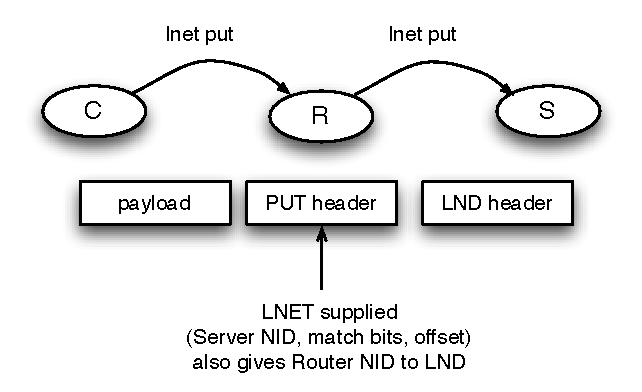
\includegraphics[width=3.5in]{img/lnet_crs}
\caption{The illustration of LNET PUT with a router in the middle scenario.}
\label{fig:crs}
\end{figure}


\subsubsection{Round 1: Client Server Interactions}

Assume that a server wants to expose a buffer to its client; below are the
steps happening on both sides, described briefly:

\begin{enumerate}

\item Server attaches the ME and MD and makes them part of some known
portal.

\item Server makes sure that the MD option is set correctly: get-only, for remote management
in this case. Now the server side is ready.

\item Client prepares the local ME and local MD for the reply if so requested.

\item Client invokes the LNET GET, with peer address, portal, match bits, etc.

\item Server receives the GET message, checks its validity (correct portal, correct
match bits, correct operation on the MD).

\item Server invokes the callback registered on the MD to notify the upper
layer. In the case of the router ping scenario we described earlier, once the
buffer is posted, the server at the upper layer may not be interested in client
requests, so this callback could just be NULL.

\item Server sends a reply message back to the client. Note that this
reply is \textbf{\textit{not}} a LNET PUT.

\end{enumerate}


\subsubsection{Round 2: More details}

\begin{enumerate}

\item Server posts a request buffer by \url{ptlrpc_register_rqbd()}. The \url{_rqbd}
is an abbrevation for request buffer descriptor, defined by the
\url{struct ptlrpc_request_buffer_desc}. It holds enough information for
creating the ME and MD. Since this is a server buffer that is to serve the request,
the matching id, as well as all important ME, MD creation is as follows:

\begin{Verbatim}
struct ptlrpc_service *service = rqbd->rqbd->rqbd_service;
static lnet_process_id_t match_id = {LNET_NID_ANY, LNET_PID_ANY};
rc = LNetMEAttach(service->srv_req_portal, match_id, 0, ~0,
                    LNET_UNLINK,LNET_INS_AFTER, &me_h);
rc = LNetMDAttach(me_h, md, LNET_UNLINK, &rqbd->rqbd_md_h);
\end{Verbatim}

\url{LNET_UNLINK} indicates this ME should be unlinked when the MD associated
with it is unlinked, and \url{LNET_INS_AFTER} means that the new ME should be
appended to the existing list of MEs. The \url{me_h} and \url{md} are defined as
\url{lnet_handle_me_t} and \url{lnet_md_t}, respectively.

\item Client sends an RPC by \url{ptl_send_rpc()}, and this function takes
\url{struct ptlrpc_request *request} as an input parameter and \textit{may}
perform the following operations:

  \begin{itemize}

  \item Client posts bulk buffer by \url{ptlrpc_register_bulk()}. This is performed
  when the bulk buffer is not NULL in the reqeust:

  \begin{Verbatim}
    if (request->rq_bulk != NULL) {
        rc = ptlrpc_register_bulk(request);
        ...
   \end{Verbatim}

  \item Client posts reply buffer by \url{LNetMEAttach()} and \url{LNetMDAttach()}.
  This operation is performed when a reply is expected (the input parameter
  \url{noreply} is set to 0).

  \item Client sends request: 
  \begin{Verbatim}
       rc = ptl_send_buf(&request->rq_req_md_h,
                          request->rq_reqmsg, request->rq_reqlen,
                          LNET_NOACK_REQ, &request->rq_req_cbid,
                          connection,
                          request->rq_request_portal,
                          request->rq_xid, 0);
  \end{Verbatim}

  \end{itemize}

\item Server handles incoming RPC by \url{request_in_callback()} defined in
\url{events.c}. This can incur two further actions:

  \begin{itemize}

  \item bulk transfer: \url{ptlrpc_start_bulk_transfer()},

  \item send reply: \url{ptlrpc_reply()}.

  \end{itemize}

\item Once the bulk transfer has been written, read, or replied to, there could be
more callback invoked such as \url{client_bulk_callback()} and
\url{reply_in_callback()}.

\end{enumerate}

\subsection{LNET API}

\subsubsection*{Naming Conventions}

Function names starting with \url{LNet} are external APIs for the upper
layers. All other functions using lower cases are internal to LNET.  Within
LNET, LND has two sets of APIs. If it starts with \url{lnd}, then it is the
API for LNET layer to call down or if it starts with \url{lnet}, then it is
for LND to call up into LNET, as illustrated in the figure below. Note that it
is confusing to use LNET to describe both as the whole network subsystem and
as a particular layer paramount to LND, but that seems the way it is being
used.

LNET compiles for both kernel space and user space. If a file is prefixed with
\url{liblnet}, it is meant for user space; otherwise, it is for kernel
space. Files under lnet/lnet are compiled twice, and those under
\url{lnet/klnds} and \url{lnet/ulnds} are compiled only once.


\begin{Verbatim}
        LNetPut      LNetGet
           |           |
      +--------------------+
      |        LNET        |
      +--------------------+               
      |     |          |   |
      |     v          v   |
      | lnd_send   lnd_recv|
      |                    |
      |        LND         |
      +--------------------+
\end{Verbatim}

\subsubsection*{Initialization and Teardown}

\url{int LNetInit(void)} and \url{int LNetFini(void)} are two APIs for
setting up and tearing down LNET connections.


\subsubsection*{Memory-Oriented Communication Semantics}

The following API has been annotated with comments:

\begin{Verbatim}
int LNetGet(
    lnet_nid_t        self,
    lnet_handle_md_t  md_in,        /* local MD to hold requested data */
    lnet_process_id_t target_in,    /* target process id */
    unsigned int      portal_in,    /* target portal index */
    __u64             match_bits_in,/* match bits used on target process */ 
    unsigned int      offset_in);   /* offset into remote MD */
\end{Verbatim}

This function initiates the remote read operation.  Note that \url{offset_in}
is only used when a target memory descriptor has the \url{LNET_MD_MANAGE_REMOTE}
flag set. It is the same for the PUT operation.

\begin{Verbatim}
int LNetPut(
    lnet_nid_t        self,
    lnet_handle_md_t  md_in,        /* local MD holding data to be sent */ 
    lnet_ack_req_t    ack_req_in,   /* flag to request Ack event */
    lnet_process_id_t target_in,    /* target process id */
    unsigned int      portal_in,    /* target portal index */
    __u64             match_bits_in,/* match bits for target process */
    unsigned int      offset_in,    /* offset into remote MD */
    __u64             hdr_data_in); /* 64-bit user data */
\end{Verbatim}

This function sends data asynchronously. The \url{self} specifies the
source NID to use and hence the outgoing NI (network interface).  If
\url{LNET_NID_ANY} is given, LNet will choose source NID and NI by itself,
based on destination NID and routing table.  Note that acknowledgments are
sent only when they are requested by the initiating process \textit{and} the
local MD has event queue \textit{and} remote MD enables them.

\subsubsection*{Match Entry Management}

\begin{Verbatim}
int
LNetMEAttach(unsigned int portal,
    lnet_process_id_t match_id, 
    __u64 match_bits, __u64 ignore_bits,
    lnet_unlink_t unlink, lnet_ins_pos_t pos, 
    lnet_handle_me_t *handle)
\end{Verbatim}

This function creates a new ME. The first parameter indicates which local
portal this ME should be associated with, and the next parameter indicates the
remote process id (or remote peer) allowed to access this ME. The rest are
match bits and ignore bits. Each portal RPC has a unique transaction id, so the
portal RPC uses this transaction id as the match bits for the reply. The
transaction id will be sent over to the remote peer, and the remote peer will
use this transaction id as the match bits in its reply buffer. The last
parameter is an ME pointer; if the call succeeds, it returns a handler.

\begin{Verbatim}
int LNetMDAttach(
    lnet_handle_me_t meh, /* ME to be associated with */
    lnet_md_t umd,        /* user-visible part of the MD */
    lnet_unlink_t unlink, /* if MD is unlinked when it is not active */
    lnet_handle_md_t *handle)
\end{Verbatim}

This function is used to create an MD and attach it to an ME. An error returns if
the ME already has an MD associated with it. \url{umd} comes from LNET client
(Portal RPC or LNET self-test for now), and it specifies parameters for the
to-be-created MD object, to which a handle will be returned in the
\url{lnet_handl_md_t *handle}.

\begin{Verbatim}
int LNetMDBind(
    lnet_md_t umd, 
    lnet_unlink_t unlink, 
    lnet_handle_md_t *handle)
\end{Verbatim}

This function creates a \textit{standalone} memory descriptor, i.e., an
MD that is not attached to an ME.

\subsection{LNET/LND Semantics and API}

LNET is connectionless, asynchronous, and unreliable. However, most LNDs are
reliable and connection-oriented such that they need to establish a connection
before they can talk to their peers. A LNET message has a payload restriction
of 1MB, \textit{and} the maximum number of segments cannot exceed 256.
Furthermore, LNET does not fragment or assemble fragments. It's assumed that
the upper layer never gives LNET a bigger payload than 1MB.  There are several
reasons for this limitation---for example the pre-set limit makes buffer
management easier and some low-level driver has a limit on the number of
scatter-gather buffers, such as 256. Also, an upper layer such as Portal RPC
can fragment data more easily if buffers are posted in pages. The downside to
this limitation is that if there is ever a network technology that supports an
MTU more than 1MB, then LNET might not be able to make full use of its
bandwidth.  \footnote{MTU is used for allocating the network bandwidth fairly.
For example, bigger MTU values might cause a malicious client to consume
the network bandwidth unfairly, while other clients might be starving.}

LND can have multiple instances---for example, in the cases where you have more
than one IB interface. Each interface is represented by a network interface
type defined by \url{lnet_ni_t}. One of the fields defined in that structure
is \url{lnd_t}---a method table callable on this particular LND type.

\subsubsection{API Summary}

LND APIs are the interface between LNET and its underlying network drivers. As
mentioned before, there are two sets of LND APIs. The first set is what LNET
expects LNDs to implement. For example, LNET expects to call LND methods to
send and receive messages. 

\begin{itemize}

\item \url{lnd_startup()}, \url{lnd_shutdown()}: These functions are called
per interface, whenever LNET wants to bring up or shut down the interfaces.

\item \url{lnd_notify()}: This is optional.

\item \url{lnd_accept()}: This is optional.

\item \url{lnd_send()}, \url{lnd_recv()}, \url{lnd_eager_recv()}: Sends
outgoing messages and receives incoming messages.

\item \url{lnd_ctl()}: This call is optional. It passes user space \url{ioctl}
commands to LND. LNET supports many ioctls through a special device file; some
are directly handled by LNET (for example, adding a route) and others must be
passed onto LND to handle.

\end{itemize}

The other set of APIs are LNET functions exported for LNDs to use:

\begin{itemize}

\item \url{lnet_register_lnd()} and \url{lnet_unregister_lnd()}: Each LND
driver calls this function to register a new LND type.

\item \url{lnet_notify()}: If a peer goes down, this function is called to
notify LNET.

\item \url{lnet_parse()}: For each new message received, LND calls this
function to let LNET know that a message has just arrived, so that LNET can
parse the message and check into it.

\item \url{lnet_finalize()}: This is called by LND on both incoming and
outgoing messages. When a message is sent, this call by LND allows LNET to
generate an event to tell that the message has been sent. For an incoming message,
this calls indicates the payload of the incoming message that has been
completely received.

\end{itemize}

\subsection{LNET Startup and Data Transfer} 

Brief notes on LNET code organizations:

\begin{Verbatim}
lnet/ulnds      /* LND in user space, */
lnet/klnds      /* LND in kernel space */
lnet/lnet       /* LNET layer */
\end{Verbatim}

Apparently, there is not much code sharing between the kernel LND and the user space
LND. Only Portals network and TCP network have an user space LND for that
reason. In the kernel space, \url{ptllnd} \footnote{For Cray SeaStar system.},
\url{o2iblnd}, and \url{socklnd} are probably the most important ones to know. 

\subsubsection{Startup}

\url{lnet_startup_lndnis()} is invoked when LNET gets initialized.

\begin{enumerate}

\item Calls on \url{lnet_parse_networks()} to parse module parameters 
provided by the user. Afterwards, LNET gets a list of network interfaces to bring
up.

\item Iterates each of the interfaces acquired above. First it tries to locate
the lnd instance represented by \url{lnd_t}. Upon finding it, it invokes the
\url{lnd_startup()}. We will look at each step in more detail.

\item Within the loop, it first looks for the driver by network type:

\begin{Verbatim}
lnd = lnet_find_lnd_by_type(lnd_type);
\end{Verbatim}

If a driver is not found, then it could be that the driver has not been loaded
yet, so it will try to load the module and then retry to locate the driver:

\begin{Verbatim}
rc = request_module(libcfs_lnd2modname(lnd_type));
\end{Verbatim}

After the driver is loaded, during its module initialization, it registers with
LNET, allowing the driver to be located later on.

\item After the driver for the network interface is located, then we can
\textit{bind} this driver to the interface and invoke the driver's startup
method:

\begin{Verbatim}
ni->ni_lnd = lnd;
rc = (lnd->lnd_startup)(ni);
\end{Verbatim}

\end{enumerate}

Now we will explain a specific LND module, socket LND. In particular, we look
into \url{ksocknal_startup()}.

\begin{enumerate}

\item If the function is being called for the first time, then it invokes
\url{ksocknal_base_startup()} to do some one-time initialization, for
example, creating the data structure shared by all interfaces.

\item Finds out which Ethernet interface to use for this network. It can be
user-specified or it can search for the first non-loopback interface in the
system.  Once located, it initializes the data structure for this interface.
The nid is generated by:

\begin{Verbatim}
ni->ni_nid = LNET_MKNID(LNET_NIDNET(ni->ni->nid),
    net->ksnn_interfaces[0].ksni_ipaddr);
\end{Verbatim}

\end{enumerate}

After LNET is initialized, a user can send or receive data on this interface.

\subsubsection{LNET Send}

We describe the general flow of the send path, starting from \url{LNetPut}
down to the LND layer.

\begin{enumerate}

\item First, the LNET message descriptor is allocated, \url{msg}, defined by
\url{struct lnet_msg_t}. This message descriptor will be passed on to LND. In
particular, there is a field within defined as \url{lnet_hdr_t msg_hdr} (the
message header) which will eventually be a part of the on-the-wire message.

\begin{Verbatim}
msg = lnet_msg_alloc();
\end{Verbatim}

\item LNET MD handle is converted from the incoming parameter to a real MD
structure, which will hold the payload:

\begin{Verbatim}
md = lnet_handle2md(&mdh);
\end{Verbatim}

\item The MD is associated with the message:

\begin{Verbatim}
lnet_commit_md(md, msg);
\end{Verbatim}

\item Message details are filled in. These details can be the type of message (PUT or GET),
match bits, portal index, offset, and user-supplied data, if any.

\begin{Verbatim}
lnet_prep_send(msg, LNET_MSG_PUT, target, 0, md->md_length);
msg->msg_hdr.msg.put.match_bits = cpu_to_le64(match_bits);
msg->msg_hdr.msg.put.ptl_index = cpu_to_le32(portal);
...
\end{Verbatim}

\item The event information is filled in as given below.

\begin{Verbatim}
msg->msg_ev.type = LNET_EVENT_SEND;
msg->msg_ev.initiator.nid = LNET_NID_ANY;
msg->msg.ev.initiator.pid = the_lnet.ln_pid;
...
\end{Verbatim}

\item Finally, lnet send function (not LND send) is invoked as below.

\begin{Verbatim}
rc = lnet_send(self, msg);
\end{Verbatim}

\item This send function needs to locate the interface to use. If the
destination is local, then it resolves to the directly attached interface. If
the destination is remote, then it resolves the interface to a router from the
routing table.  The result of this search is \url{lp}, defined by \url{struct
lnet_peer_t}, representing the best choice of a peer. This peer can be either
the interface for the router or the interface for the final destination as
below.

\begin{Verbatim}
msg->msg_txpeer = lp;
\end{Verbatim}

\item Next, \url{lnet_post_send_locked()} is called for credit checking.
Suppose you are only allowed to send $x$ number of concurrent messages to the
peer. If you exceed this credit threshold, the message will be queued until
more credits are available.

\item If credit checking passed, then:

\begin{Verbatim}
if (rc==0)
    lnet_ni_send(src_ni, msg);
\end{Verbatim}

This send function invokes LND send for further sending:

\begin{Verbatim}
rc = (ni->ni_lnd->lnd_send)(ni, priv, msg);
\end{Verbatim}

At some later point, after LND finishes sending the message,
\url{lnet_finalize()} will be called to notify the LNET layer that the message
is sent. However, let's continue down the path of sending data. Let's assume it
is an IP network; then socket LND send, more specifically,
\url{ksocknal_send()} will be called. 

\item Remember that socket LND is connection based, so when you want to send
something, first you need to locate the peer, then you have to check if a
connection has been established. If there is one, you just queue the \url{tx}
to the connection.

\begin{Verbatim}
if (peer!=NULL) {
    if (ksocknal_find_connectable_route_locked(peer) == NULL) {
        conn = ksocknal_find_conn_locked(tx->tx_lnetmsg->msg_len, peer);
        if (conn != NULL) {
            ksocknal_queue_tx_locked(tx,conn);
            ...
 }
\end{Verbatim}

So eventually, the message queued will be sent on the socket connection
through the kernel socket API. 

\item If there is no connection yet, then we queue the message to peer first,
so that when a new connection is established, we can move the message from the 
peer's queue to the connection's queue to be sent out.

The message format sent on the wire has the following layout, briefly:

\begin{Verbatim}
 +--------------+-----------+-----------------+-------------+-----------+
 | TCP, IP, and | sock LND  | LNET msg type   | LNET common |  payload  |
 | MAC header   | header    | specific header | header      | (from MD) |
 +--------------+-----------+-----------------+-------------+-----------+
\end{Verbatim}

\item There are two ways (APIs) to send a message from socket LND: If the
message is small, normal send will put the message into a kernel socket
buffer (each socket has a send buffer). This is \textit{not} a zero-copy
transfer.  Alternatively, you could send this buffer directly onto the network
without making a copy first (zero copy transfer). However, zero-copy has its
own overhead, so Lustre only utilizes this path for large messages.

\end{enumerate}


\subsubsection{LNET Receive}

On the receiving end, assuming that we are using socket LND, 
\url{ksocknal_process_receive()} is the entry function for receiving. The
general steps are given here.

\begin{enumerate}

\item LND starts to receive the new message. At first, it only receives up to LNET
message header because it doesn't know where to put the payload yet, only LNET
layer has the information on the destination MD.

For this reason, LND gives LNET header to \url{lnet_parse()}. This function
LNET layer will look into the header and identify the portal, offsets,
match bits, source NID, source PID, etc. LNET can either reject the message (for
example, malformed) or accept it.

\item If proper MD is located, LNET (from \url{lnet_parse()} calls another
LND API,  \url{lnd_recv()}. Now the payload from the socket kernel buffer is copied
over to the destination MD. In the case of socket LND, this is one kernel
memory-to-memory copy.
 

\item LNET calls \url{lnd_eager_recv()} immediately if it will call \url{lnd_recv()}
sometime later.

\item After LNET calls \url{lnd_recv()}, LND starts receiving the payload
(either by memory-to-memory copy or RDMA) and LND should call
\url{lnet_finalize()} within a finite time. LND could use RDMA for data
transfer at this point if it is available.

\end{enumerate}

Also note that TCP can perform fragmentation, but when \url{lnd_recv()}
finishes, it delivers the complete message, after de-fragmenting the message.

\subsubsection{The Case for RDMA}

We have mentioned that there is a memory-to-memory copy in socket LND. For any
RDMA supporting network, for example, o2ib LND, it would RDMA data directly
into destination MD, therefore avoiding the memory-to-memory copy. More complete
interactions are as follows:

\begin{enumerate}

\item LNET PUT passes the message to o2ib LND. Now o2ib LND has two pieces of
information: An LNET message header, which holds information such as source NID and
destination NID, and an MD pointing to the actual payload.

\item Unlike socket LND, o2ib LND only sends (using OFED API) the LNET header
over the network to the peer. The message includes an o2ib LND header, which
indicates this is an o2ib PUT request. 

\item At the receiving end, o2ib LND still calls \url{lnet_parse()} as it has
the LNET header information and it identifies the MD. Then it calls
\url{lnd_recv()} to receive the data. o2ib's \url{lnd_recv()} will register
the MD buffer with OFED first. After the memory is registered, it gets an OFED
\textit{memory ID}, which identifies the registered memory.

\item Now o2ib sends another message (PUT ACK) back to the initiator, along
with the remote memory ID. The initiator registers this message with its
local MD holding the payload and gets a local memory ID. Finally, it calls on
\url{RDMA write} and passes the control to OFED for further processing.

\end{enumerate}

\subsection{LNET Routing}

\subsubsection*{General Concepts}

There are two basic characteristics about Lustre routing. First, all nodes
inside a Lustre network can talk to each other directly without any involvement
from the routing layer. Second, Lustre routing is static routing, where its
network topology is statically configured and parsed when the system
initializes.  Configuration can be updated at the runtime and the system
responds to it, however, this ``dynamic update'' is very different from
distance vector or link state based routing as we know it. 


A crude definition of a Lustre network would be \textit{a group of nodes that
can communicate with each other directly without involvement of routing}. Each
Lustre network has a unique type and number, for example, tcp0, ib0, ib1, etc.,
and each end node has an NID (Network Identifier). Figure
\ref{fig:lnet_topology} illustrates a sample LNET routing layer stack. Here are
some artifacts of this definition: (1) It has nothing to do with IP subnet and
IP router. So if you have two networks that have an IP router in between, it
\textit{can} still be considered one Lustre network. (2) If you have one end
node with TCP interface and another end node with IB interface, then you must
have an LNET router in between, and this will be considered two Lustre
networks. (3) The addresses within a Lustre network must be unique.  

Another implication of the above definition is that the routing table of an end node
will have LNET router as its next hop, not the IP router. To specify a Lustre
network, you typically use one of two directives: \url{networks} or \url{ip2nets}: 

\begin{Verbatim}
    # router
    options lnet networks = tcp0(eth0), tcp1(eth1)
    # client
    options lnet networks = tcp0
    # single universal modprobe.conf
    options lnet ip2nets="tcp0(eth0,eth1) 192.168.0.[2,4]; tcp0 192.168.0.*; \
        elan0 132.6.[1-3].[2-8/2]"
\end{Verbatim}


\begin{figure}[htb]
\centering
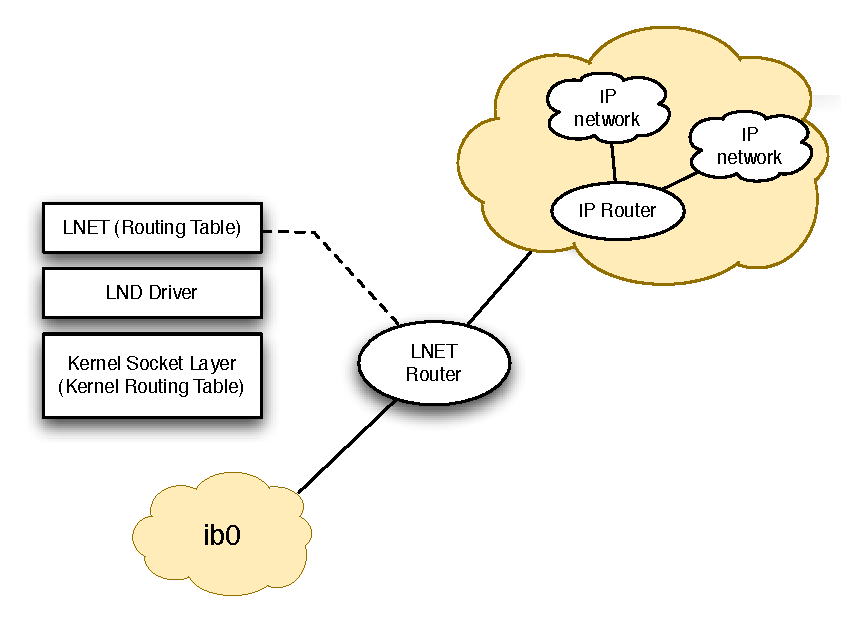
\includegraphics[width=4.5in]{img/lnet_topology}
\label{fig:lnet_topology}
\caption{Illustration of LNET routing layer stack.}
\end{figure}


\subsubsection{Asymmetric Routing Failure}

This topic highlights a deficit we discovered in the current LNET production code. It is
pertinent to the general discussion on LNET, and
we believe it would be good to share our observation with a broader audience. The problem is
that it can be difficult for a router to reliably determine if an interface is
down. Right now, LNET does not even try to do it. So for a configuration
where a router has two interfaces, such as \url{tcp0} and \url{ib0}, if the \url{ib0}
interface is down and end nodes connected with \url{tcp0} are still pushing
data, this will result in an intermittent communication failure.

One idea towards solving this problem is that the  LNET router can try to
detect the transmission problem, then temporally disable all its interfaces. A
router might be able to do this more intelligently by disabling only some
interfaces if it has information on the full topology and the incoming path
that clients use. Until then, shutting down all of its interfaces seems to be
better than suffering timeout as a result of intermittent communication
failure.

\subsubsection{Routing Buffer Management and Flow Control}

Upon initialization, an LNET router pre-allocates a fixed number of routing
buffers. The LNET layer of an end node won't need to do this (except when
initializing its routing tables). Allocating and managing routing buffers are
the primary, if not the only, difference between the execution logic of an end
node and a router.

As routing buffers are limited resources, to prevent a single end node from
overwhelming a router, each end node is given a quota. Once a buffer has been
forwarded, it can be recycled again. The quota for each end node is also known
as \textbf{buffer credit}. It is only significant for routers, and it is
different from the ``RPCs in flight" credit, which is known as \textbf{peer to
peer credit}. One RPC can involve several LNET messages (at most ten), and these
can be one request LNET message, one reply LNET message, and in the case of a
bulk transfer, there could be four LNET messages going one way, and four LNET
messages going in the opposite direction. This also implies that the bulk
transfer LNET messages are part of the bulk RPC transaction, but they are
\textbf{not} considered an RPC. Therefore, they (the four bulk transfer messages)
are not counted towards RPCs in flight.

There are three kinds of router buffers: 1MB (maximum amount of payload an LNET
message can carry), 4KB for small messages, and zero payload buffers for tiny
messages such as ACK. 

Requests from an end node are on a first come, first served basis. If requests from
a particular end node exceed its quota, then its next request will not be
handled until the router buffer is freed, which is essentially the way LNET
layer does flow control (flow control is point-to-point). It is up to the upper
layer to implement an end-to-end flow control, for example, by number of RPCs
in flight. The buffer can be freed when the underlying LND calls the
\url{lnet_finalize()} as an indication that LND considers the forwarding done,
but it doesn't really mean the message has been put on the wire. Depending on
the size of the message, LND and kernel may have different logics for handling
it. The only requirement from LNET is, once \url{lnet_finalize()} is invoked,
LNET should be able to recycle the buffer freely. 

Logically, LNET has a single queue, and incoming messages from all interfaces
are queued and processed in order. Each interface has its own interface
queues; however, that is not a concern of LNET since this is interrupt-driven.
So it is guaranteed that each incoming message is handled in the order it
arrives.  


\subsubsection{Fine Grain Routing}

This feature is a recent development (Lustre bug \#15332) for Jaguar/Spider
deployment at ORNL. The motivation is that LNET doesn't assign weights to
routes. So if you have multiple routers that reach the same destination,
LNET will perform a round robin algorithm to distribute the load, and this
applies to both end node and router. What fine grained routing adds, is simply,
to assign weights to different routers, preconfigured by the system
administrator.  The goal is that \textit{better} routes gets more traffic.
Here, better is defined by the site system administrator.

\begin{Verbatim}
   dest network 1:
        w1    (router 1, router 3)
        w2    (router 4, router 5)
        w3    (router 2)
\end{Verbatim}

So for example, you can specify different weight classes and assign routers to
each to indicate your preference. If $w_1 < w_2$, then $w_1$ is the preferred
weight class of the two. Within a given weight class, routers are equal.

More specific to our case, this mechanism provides the potential for a client
to pick a router closer to its proximity as its preferred router.


%\section{Infrastructure Support}

This section discusses miscellaneous aspects related to Lustre initialization,
client registration, obd devices management, etc.

\subsection{Lustre Client Registration}

Lustre client side or Lustre Lite registers as a filesystem with the name
``lustre.''  The file system type is defined as:

\begin{Verbatim}
    struct file_system_type lustre_fs_type = {
        .owner      = THIS_MODULE,
        .name       = "lustre",
        .get_sb     = lustre_get_sb,
        .kill_sb    = lustre_kill_super,
        .fs_flags   = FS_BINRARY_MOUNTDATA | FS_REQUIRES_DEV 
                        LL_RENAME_DOES_D_MOVE,
    };
\end{Verbatim}

Another function defined by \url{lustre_register_fs()} simply invokes kernel
function:

\begin{Verbatim}
    return register_filesystem(&lustre_fs_type);
\end{Verbatim}

and will be done with the registration. This was invoked when \url{obdclass} as
a module was being initialized.
 
\begin{Verbatim}
int init_obdclass(void) {
...
#ifdef __KERNEL__
    err = lustre_register_fs()
#endif
}
\end{Verbatim}

See \url{class_obd.c} for more details.

\subsection{Superblock and Inode Registration} 

It should be a relatively simple matter, but Lustre jumps through several hoops
that may be due to some legacy support issues.

When Lustre Lite initializes as a Linux module, \url{init_luster_lite()} was
defined in \url{super25.c} \footnote{It is actually used for Linux Kernel 2.6 as well.} 
Among things such as allocating inode cache, it assigns (essentially)
the function pointer \url{*client_fill_super} with \url{ll_fill_super}.

In the \url{luster_fill_super()} method, we check if this is a client mount.
If it is, it makes calls to \url{(*client_fill_super)(sb)}, where \url{sb} is
the superblock.


\subsection{OBD Device}

OBD device is meant to provide a level of abstraction on Lustre components such
that the generic operations can be applied without knowing the specific devices
you are dealing with. We discussed the method tables defined on it in Section
\ref{sec:ost-and-obdfilter}. Lustre also provides some generic infrastructure
for managing object devices. The core structures are \url{obd_devices} and
\url{exports}. We discuss them in detail.

Each obd device was assigned an integer number, there are at most
\url{MAX_OBD_DEVICES} obd devices that can be created on a given node. You can retrieve an
obd device through an integer number (\url{obd_minor}), a name, or a uuid. All obd
devices are stored in an array internally. However, the preferred way to
retrieve an obd device is through a set of API as discussed below.

\begin{comment}
OBD device can be clustered into a group, in that case, they will share
a common group id.
\end{comment}

\begin{Verbatim}
struct obd_device *obd_devs[MAX_OBD_DEVICES]
\end{Verbatim}

The API can be roughly divided into five categories:

\begin{itemize}

\item Register and unregister a device type.

\item Allocate and free obd devices. \url{obd_device_alloc()},
\url{obd_device_free()}.


\item Create and release obd devices. You can create new obd devices
by giving a string type and string name through \url{class_newdev()}. 
You can release one by giving a pointer to \url{obd_device} that it is to be
released. In both cases, they internally invoke allocation and free
functions.

\item Search. You can search by type through \url{class_search_type()}; 

\item Conversion utilities.

\end{itemize}


\subsection{Import and Export}

For two OBD devices $A$ and $B$ to communicate, they need an import and export
pair: $A_{import}$ and $B_{export}$. $A_{import}$ is for sending requests and
receiving replies, and $B_{export}$ is for receiving requests and sending
replies.  However, the same pair cannot be used the other way around: that is 
you cannot send a request through $B_{export}$. For that to happen, such as in
the case of sending ASTs, you need so-called ``reverse import.'' Essentially,
reverse import converts the $A_{import}$ and $B_{export}$ pair into an $A_{export}$
and $B_{import}$ pair. The need for establishing such a pair at OBD
devices is partially illustrated in Figure \ref{fig:exp}.


\begin{figure}[htb]
\centering
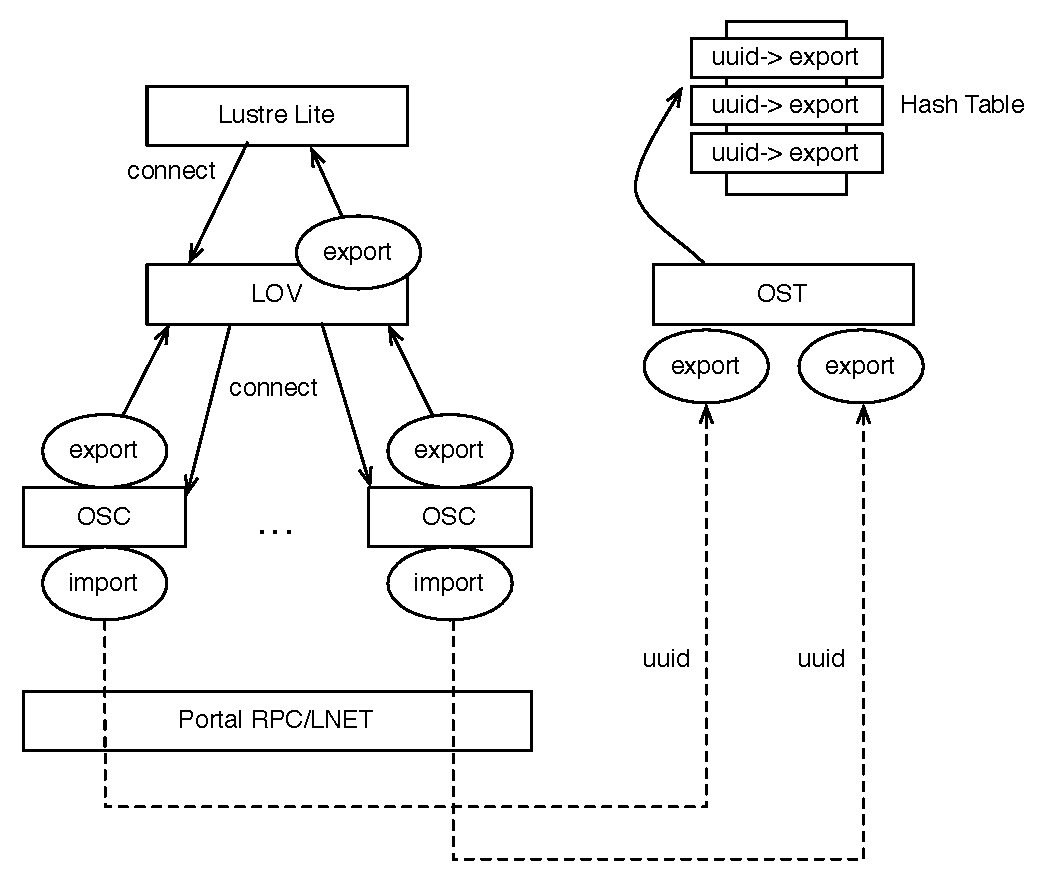
\includegraphics[width=4.5in]{img/lustre_exp}
\caption{Setup export and import.}
\label{fig:exp}
\end{figure}

Note that LOV, OSC, and OST in the figure are all defined as types of OBD
devices.

%%%%%% this figure is kinda of duplicate of above one 
%%%%%%
\begin{comment}

\begin{figure}[hbt]
\centering
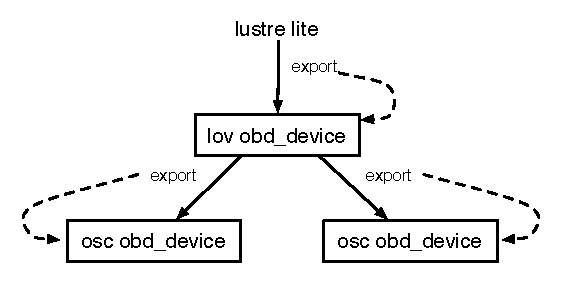
\includegraphics[width=3in]{img/exports}
\end{figure}

\end{comment}


\begin{comment}
\section{Debugging Lustre}

\subsection{Tracing}

We can learn the call sequences by turning on all debug traces of
Lustre. The following steps detail how by looking at a simple touch
operation.

\begin{Verbatim}
ictl    clear                       # clear previous log
echo -1 > /proc/sys/lnet/debug      # turn on all debugs
touch /mnt/lustre/fwang2.img
lctl dk > /tmp/touch.trace          # dk -> dump kernel
\end{Verbatim}

\end{comment}


\section{Lustre Numbers}

Anything to do with number is of interests here.


\begin{itemize}

\item Stripe Information

\begin{Verbatim}
    # -s 0  : default stripe size, otherwise, multiple of 64KB
    # -i -1 : random first OST is chosen, 0 to N-1 is OK
    # -c -1 : all available OSTs are used; 0 if default number of OSTs  
    lfs setstripe -s 0 -i -1 -c -1
\end{Verbatim}

\item Free space management: weighted allocator is used when any two OSTs are
imbalanced by more than 20\%. Until then, roound robin allocator is used.

\begin{Verbatim}
    lctl conf_param <fsname>-MDT0000.lov.qos_prio_free=90
\end{Verbatim}


\item Client 32-bit checksum is enabled by default:

\begin{Verbatim}
    echo 0 > /proc/fs/lustre/llite/{fsname}/checksum_pages
\end{Verbatim}


\item OST limit right now is 8TB, and it will be 16TB when ldiskfs migrates to
ext4. 

\item MDT device can be up to 8TB in size. With default configuration, you get
one inode for every 4KB, but you can double the inodes if you format it with
one inode every 2KB.

\item Dirty cache limit on a per-OSC basis is tunnable by \url{max_dirty_mb},
default is 3/4 of RAM.

\begin{quote}

\url{get_param} and \url{set_param}: Up to 1.6.5, these two \url{lctl} actions
are supported, and is a preferred way to doing parameter changes than querying
the \url{/proc}. An example Andreas gave is:
\smallskip
\begin{Verbatim}
lctl set_param osc.*.max_dirty_mb = 512
\end{Verbatim}
\smallskip
instead of:
\smallskip
\begin{Verbatim}
for x in /proc/fs/lustre/osc/*/max_dirty_mb; do
    echo 512 > $x
done
\end{Verbatim}

\end{quote}

\item Dirty cache limit per client:
\url{/proc/fs/lustre/llite/*/max_cached_mb}, default is 32MB.


\item Read ahead, default size is 40MB

\item OSS cache (1.8 release), the tunable
\url{/proc/fs/lustre/obdfilter/*/readcache_max_filesize} will limit the
maximum file size that is cached on the OSS so that small files can be cached,
and large files will not wipe out the read cache.



\item To find out what network/IP address is provisioning which OST target,
or MDT target for that matter.

\begin{Verbatim}
lctl get_param osc.${fsname}-${OSTname}*.ost_conn_uuid
lctl get_param mdc.${fsname}-${MDTname}*.mds_conn_uuid
\end{Verbatim}

There will be a \url{lct list_param} command in upcoming release to get all
valid parameters you can play.


\item The number of client currently mounted? Check
\url{/proc/fs/lustre/mds/num_exports}. Note that each server has an internal
reference to the device, so this file is number of clients plus 1.


\item The largest memory ever used by the Lustre code itself? check
\url{lustre.memused_max} parameter.


\end{itemize}







\end{document}
